% M. S. Tsoeu (2011), University of Cape Town <mohohlo.tsoeu@uct.ac.za>

% This is a project report templace document created for EEE4022FS students at the University of Cape Town.
%
% This file should be is processed with ``pdflatex`` and might need a few modifications if a different processor is chosen.


\documentclass[a4paper,12pt]{report}

%Include packages you need to use here

%\usepackage[top = 1in, bottom = 1in, left = 1in, right = 1in]{geometry}
\usepackage[a4paper, margin=25mm, headheight=15pt, headsep=7mm, footskip=10mm]{geometry}
\usepackage{graphicx}
\usepackage{fancyhdr}
\usepackage{amsmath, amsthm, amssymb}
\usepackage{lastpage}
\usepackage{lscape}
\usepackage{hyphenat}
\usepackage{setspace}
\usepackage{titlesec}
\usepackage{enumitem}

% Keeps the two-line "Chapter N / Title" look, just smaller and tighter
\titleformat{\chapter}[display]
{\normalfont\bfseries}          % overall format
{\Large\chaptertitlename\ \thechapter} % "Chapter 3"
{8pt}                           % gap between "Chapter 3" and the title
{\huge}                        % title size
\titlespacing*{\chapter}{0pt}{0pt}{16pt}  % {left}{space above}{space below}

\usepackage{hyperref}
\usepackage{pgfplots}
\usepackage{float}
\usepackage{booktabs}
\usepackage{longtable}
\usepackage{siunitx}
\usepackage{subcaption}
\usetikzlibrary{arrows.meta,positioning,calc,decorations.markings,fit,backgrounds,patterns,decorations.pathmorphing}
\pgfplotsset{compat=1.18}


% Include page formatting here. 
\parskip = 4mm
\parindent = 0mm
\renewcommand{\headrulewidth}{0pt}
\rhead[]{\thesection}
\lhead[\thechapter]{}


\begin{document}
 
% This section formats the title page of the Report.
\thispagestyle{empty}
{\Huge \begin{center}
% Modify the line below to insert your title.
Insert your title here
\hrule 
% Modify the line below to insert your subtitle.
{\Large Insert a subtitle here (if applicable)}
\end{center}}

\vskip 5mm
\begin{center}
\- \- \- \- \- \- \- \- \- \-
\includegraphics[scale = 0.3]{uctLogo.png}
\end{center}

\vskip 5mm
\begin{center}
Presented by:\\
Mohohlo Samuel T\v soeu		% Insert your name here
\end{center}

\vskip 10mm
\begin{center}
Prepared for:\\
M. S. T\v soeu\\ 		% Insert your supervisor's name here.
Dept. of Electrical and Electronics Engineering\\University of Cape Town
\end{center}


\vskip 10mm
\begin{center}
Submitted to the Department of Electrical Engineering at the University of Cape Town in partial
fulfilment of the academic requirements for a Bachelor of Science degree in ***INSERT DEGREE
NAME HERE (Electrical Engineering; Mechatronics or Electrical and Computer Engineering)

\end{center}


\vskip 5mm
\begin{center}{\bf \today}
\end{center}

\newpage
\thispagestyle{empty}
\mbox{}
\newpage

\onehalfspacing

\thispagestyle{empty}
\vskip 40mm


% Please leave the declaration as it is (Standard UCT declaration).
{\Large Declaration}\\
\hrule

\vskip 10mm
\begin{enumerate}
	\item I know that plagiarism is wrong. Plagiarism is to use another's work and pretend that it is one's own.
	\item I have used the IEEE convention for citation and referencing. Each contribution to, and quotation in, this report from the work(s) of other people has been attributed, and has been cited and referenced. Any section taken from an internet source has been referenced to that source.
	\item This report is my own work, and is in my own words (except where I have attributed it to others).
	\item I have not paid a third party to complete my work on my behalf. My use of artificial intelligence software in this report has been limited to formatting of tables, figures and plots, as well as error checking and assistance in clarity and conciseness. See examples of prompts in Appendix \ref{appendix:AIUse}. 
	\item I have not allowed and will not allow anyone to copy my work with the intention of passing it off as his or her own work.
	\item I acknowledge that copying someone else's assignment or essay, or part of it, is wrong, and declare that this is my own work.
\end{enumerate}

\vskip 10mm
Signature: Thomas Bingle Kruger 		% Chante this line to your name.
\vskip10mm
Date: \today.

\newpage
\thispagestyle{empty}
{\Large Terms of Reference}\\
\hrule

The terms of reference page is an agreement between yourself and your supervisor outlining what is expected of you in your final year project. Please make sure that this is discussed and written at the beginning of your thesis project. 


\fancyfoot[C]{\thepage}
\pagestyle{plain}
\newpage
\pagenumbering{roman}
{\Large Acknowledgments}\\
\hrule
Make relevant acknowledgements to people who have helped you complete or conduct this work, including sponsors or research funders.


\newpage

{\Large Abstract}\\
\hrule

% Place your abstract here.
\begin{itemize}

\end{itemize}


\newpage
\tableofcontents

%\newpage
%\listoffigures

%\newpage
%\listoftables

% Page formatting, to place section titles as headers of odd pages and Chapter titles as headers of even pages.
\newpage
\fancyhead[RE,LO]{}
\fancyhead[LE]{\leftmark}
\fancyhead[RO]{\rightmark}
\pagestyle{fancy}

\pagenumbering{arabic}

% THe files included below are .tex files containing the respective chapters these are already created in this package and you can add to or modify them.
\chapter{Introduction}

\section{Background to the study}
Wind has become a mainstream source of electricity. A record 165\,GW of
new wind capacity was installed worldwide in 2025, 40\% more than the
previous record year, bringing cumulative capacity to roughly 1.3\,TW
across 138 countries \cite{gwec2026}. Delivering that growth at acceptable cost depends on how well the wind
resource itself can be characterised, which Veers et al. identify as one
of the grand challenges of wind energy science \cite{veers_grand_2019}.
Wind speed is an important factor in analysis of a turbine's economics
and engineering. The power available in the wind scales with the cube of
wind speed, so a small error in measured or predicted wind speed becomes
a much larger error in predicted energy \cite{windenergyhandbook}. Furthermore, wind speed and turbulence significantly affect the structural fatigue on a turbine, and act as an input to controllers which control the pitch and yaw of the turbines appropriately to maximise power generation and minimise stresses on the structure. It is clear that real-time measurement of the wind field around wind-turbines is a critical objective for this industry, and one to which much attention must be given. However, turbines operate in the lower atmospheric boundary layer, where the flow
is turbulent and shaped by mesoscale circulation, orography, thermal stratification and the wakes of neighbouring turbines, which makes this characterisation of the wind-field difficult \cite{letizia_characterization_2023}.

The traditional instrument for wind-speed measurement for wind-turbines is the meteorological mast (met-mast),
which holds cup and sonic anemometers at fixed heights, mounted on a long mast. This technology is well established, providing high resolution measurements, and indeed acting as a reference point to which any alternative method is compared \cite{liu_review_2019}, \cite{hill_remote_nodate}. This methodology however holds several limitations:

Erecting a meteorological mast can be costly, particularly for offshore wind-turbines \cite{wagner_uncertainty_2016}. Once constructed, the  met-mast is naturally limited to a single location, which limits spatial coverage - this makes variability in the wind, which occurs over larger areas, difficult to characterise \cite{letizia_characterization_2023}. Furthermore, the wake of the mast itself can corrupt measurements in the anemometer \cite{letizia_characterization_2023}. These constraints motivated the research into a remote sensing alternative to in-situ measurements.

Advancements in LiDAR technology have resulted in the technology presenting an alternative and/or complement to existing wind-speed measurement techniques. This allows for the development of new turbine control and assessment strategies, which overcome some of the limitations of traditional wind-speed measurement techniques. 

Doppler wind LiDAR (DWL) systems measure the line-of-sight velocity of wind by emitting a laser beam into the atmosphere and measuring the Doppler shift of the beam after being backscattered by naturally occurring aerosols and particles (see \autoref{sec:lit-principlesDWL}). There are numerous commercial DWL systems available, such as Qinetiq's ZephIR whose first deployment was on the nacelle of a 2.3\,MW turbine, and with Vaisala's (formerly Leosphere) pulsed WindCube shortly afterwards \cite{hill_remote_nodate} \cite{cariou_leosphere_nodate}. Letizia et al. identified several promising application areas for nacelle-mounted LiDAR (NML) systems, including load reduction, performance optimization, and performance assessment \cite{letizia_characterization_2023}. NML systems present several advantages over traditional measurement techniques for these ends, including larger field of view and spatial coverage (particularly for scanning LiDARs) and reduced costs and maintenance \cite{letizia_characterization_2023}.

Despite this however, scientific access to these systems is limited by high
costs, with commercially available systems being quote-only, and estimated in the range of tens to hundreds of thousands of USD. Simley et al. identify system cost, alongside availability and reliability, as one of the principal barriers to the wider adoption of LiDAR for wind-turbine applications \cite{simley_optimizing_2018}. Furthermore, commercial instruments are sold as complete, pre-calibrated products, so the design choices within them, and the effect of each choice on the system's noise and sensitivity, are not open to examination by the user. For universities and smaller research groups, this places both the instruments and an understanding of their internal trade-offs largely out of reach. It was these reasons which thus motivated this study into DWL system design within a more resource constrained environment, where there are more limitations on component availability and cost than in a commercial enterprise. Trade-offs in system design and functionality need to be carefully balanced with respect to the resources at hand, so as to gain an understanding of the internal workings and limitations of these systems.

 
\section{Objectives}
The primary objectives of this project are to design, build, and test a Doppler Wind LiDAR system from readily available parts and components. This is done with the intention of illustrating clearly the principles involved in the design of such a system, and to make system performance in test environments attributable to design and component choices. From this a greater scientific understanding of such systems can be gained, particularly with respect to their limitations when designed and built with resource constraints. The system is not intended to form a fully functional, field-ready DWL system, with the final performance objective being limited to a benchtop-scale system, which fulfills performance requirements and illustrates the system's working principles in a constrained lab environment. The tests which are performed on the system must however illustrate a clear upgrade-path for the system, and quantify the degree of performance of the current system, and the degree which is required for real-world use. 

\section{Scope and Limitations}
The project's scope chiefly concerns the photonics, optics, and electronics-level design of a DWL system. This includes the overall choice of architecture of the system, as well as the individual components which make up the system. There are however several limitations imposed on the design of the system, and the overall scope of the project:

\begin{itemize}
	\item \textbf{Final system performance:} As noted previously, the system is not intended, nor expected, to be usable outside of a controlled lab environment in the form presented at the conclusion of this project. However, system performance in the lab must be quantified and thoroughly investigated. \\
	\item \textbf{Component cost and availability:} The system will be limited by the cost and availability of the highly specialised components required. While a strict budget is not provided, components costs are evaluated on a case-by-case basis to determine if omission or a lower-cost option is feasible for this benchtop-scale system. The system was thus kept as simple and inexpensive as possible, given the high cost typically associated with photonics equipment. \\
	\item \textbf{Data acquisition and processing:} Acquisition and processing of the system's outputs are naturally required to test the system, and will be performed. However, this project is not concerned with \textbf{real-time} processing of the data, as indeed, this aspect is of enough complexity to warrant an entirely separate project. Instead, simple lab equipment is to be used for data acquisition to simplify the system and reduce costs, and a laptop is used for post-processing of data. The system may be extended in a future iteration to include real-time processing functionality. \\
	\item \textbf{Housing:} While a suitable housing and test-rig will be designed for the system to be used in a lab environment, this project is not concerned with the design of a robust housing which would allow for weather protection and mounting on the nacelle of a turbine. \\
\end{itemize}

\section{Report outline}
Following this brief introduction to the background and scope of the study, \autoref{sec:litReview} reviews the literature concerned with the principles of DWL systems, including various architectue types and design considerations identified by current research. Thereafter \autoref{sec:systemDesign} details the choice of architecture, the system requirements, and the design decisions made for this project from the reviewed literature and the objectives and scope of the project. \autoref{sec:noiseAnalysis} gives a comprehensive analysis of noise in the system, which informs a substantial component of the system's overall performance. \autoref{sec:functionalTesting} performs various functional tests on the system, and analyses its functional performance in a lab environment. Finally \autoref{sec:conclusionAndRecommendations} gives concluding remarks based on the tested performance of the system, and gives recommendations for future iterations and extensions of the system, particularly with respect to obtaining a system which is capable of wind-speed measurement for application in the wind energy sector. 

% =====================================================================
%  Literature Review
% =====================================================================

\chapter{Literature Review}
\label{sec:litReview}

% ---------------------------------------------------------------------
\section{Wind Measurement in the Wind Energy Sector}
    \subsection{Introduction}
    Wind has become a mainstream source of electricity. A record 165\,GW of
    new wind capacity was installed worldwide in 2025, 40\% more than the
    previous record year, bringing cumulative capacity to roughly 1.3\,TW
    across 138 countries \cite{gwec2026}. Delivering that growth at acceptable cost depends on how well the wind
    resource itself can be characterised, which Veers et al. identify as one
    of the grand challenges of wind energy science \cite{veers_grand_2019}.
    Wind speed is an important factor in analysis of a turbine's economics
    and engineering. The power available in the wind scales with the cube of
    wind speed, so a small error in measured or predicted wind speed becomes
    a much larger error in predicted energy \cite{windenergyhandbook}. Furthermore, wind speed and turbulence significantly affect the structural fatigue on a turbine, and act as an input to controllers which control the pitch and yaw of the turbines appropriately to maximise power generation and minimise stresses on the structure. It is clear that real-time measurement of the wind field around wind-turbines is a critical objective for this industry, and one to which much attention must be given. However, turbines operate in the lower atmospheric boundary layer, where the flow
    is turbulent and shaped by mesoscale circulation, orography, thermal stratification and the wakes of neighbouring turbines, which makes this characterisation of the wind-field difficult \cite{letizia_characterization_2023}.
    

    \subsection{Current In-Situ Anemometry Methods and Limitations}
    The traditional instrument for wind-speed measurement for wind-turbines is the meteorological mast (met-mast),
    which holds cup and sonic anemometers at fixed heights, mounted on a long mast. This technology is well established, providing high resolution measurements, and indeed acting as a reference point to which any alternative method is compared \cite{liu_review_2019}, \cite{hill_remote_nodate}. This methodology however holds several limitations:

    Erecting a meteorological mast can be costly, particularly for offshore wind-turbines \cite{wagner_uncertainty_2016}. Once constructed, the  met-mast is naturally limited to a single location, which limits spatial coverage - this makes variability in the wind, which occurs over larger areas, difficult to characterise \cite{letizia_characterization_2023}. Furthermore, the wake of the mast itself can corrupt measurements in the anemometer \cite{letizia_characterization_2023}. These constraints motivated the research into a remote sensing alternative to in-situ measurements.
    
    
% ---------------------------------------------------------------------
\section{LiDAR as an Alternative}

    \subsection{Introduction}
    Advancements in LiDAR technology have resulted in the technology presenting an alternative and/or complement to existing wind-speed measurement techniques. This allows for the development of new turbine control and assessment strategies, which overcome some of the limitations of traditional wind-speed measurement techniques. 

    Doppler wind LiDAR (DWL) systems measure the line-of-sight velocity of wind by emitting a laser beam into the atmosphere and measuring the Doppler shift of the beam after being backscattered by naturally occurring aerosols and particles (see \autoref{sec:lit-principlesDWL}). There are numerous commercial DWL systems available, such as Qinetiq's ZephIR whose first deployment was on the nacelle of a 2.3\,MW turbine, and with Vaisala's (formerly Leosphere) pulsed WindCube shortly afterwards \cite{hill_remote_nodate} \cite{cariou_leosphere_nodate}. Research has been focused on two areas; ground-based systems for wind-speed measurement (primarily for resource assessment prior to building wind-energy farms), and nacelle-mounted LiDAR (NML) systems \cite{letizia_characterization_2023}. 
    
    Letizia et al. identified several promising application areas for NML systems, including load reduction, performance optimization, and performance assessment \cite{letizia_characterization_2023}. NML systems present several advantages over traditional measurement techniques for these ends, including larger field of view and spatial coverage (particularly for scanning LiDARs) and reduced costs and maintenance \cite{letizia_characterization_2023}. The following subsections provide a brief overview of different NML application areas, and progress and limitations in these sectors. These areas of research present viable means to lower the levelized cost of energy (LCOE) for wind-turbines, and are thus well-suited to the growing demands for wind-energy systems globally \cite{letizia_characterization_2023}. 

    \subsection{NML for Load Reduction}
    Wind gusts can place significant load on a wind-turbine structure - however appropriate control of the turbine's rotor pitch can serve to decrease this load, preserving the structural integrity and longevity of the system.
    Standard turbine controllers are feedback systems that react to
    a turbulent gust only after it has loaded the rotor. A lidar preview of
    the approaching wind-field however would enable feed-forward pitch action \textbf{before} the gust
    arrives, and there is consensus that load reduction in certain regions of wind-turbine operation is a promising lidar-assisted control
    (LAC) application \cite{letizia_characterization_2023}. Crucially however, any benefit from feedforward LAC for load-reduction is limited by
    the coherence between the wind-speed measured by the LiDAR from a distance, and the actual wind-speed which hits the turbine rotors (rotor-effective wind-speed) \cite{letizia_characterization_2023}. The seminal simulation study of Harris et al. reported a 10\% reduction
    in damage-equivalent load on the flapwise blade root \cite{harris2006}, which spurred on further research into the topic. There is much ongoing research on the topic, particularly with respect to the evolution of the wind-field in between sensing and reaching the turbine, and reported results span a wide range. This lack of consolidation has thus presented a barrier to widespread adoption of LAC for load reduction, however research thus far indicates that this is indeed a promising application of the technology \cite{simley_optimizing_2018} \cite{letizia_characterization_2023}. 
    
    \subsection{NML for Performance Optimization}
    Another application area for LAC is performance optimization, where feedforward control based on NML measurements of the incoming wind-field can be used to yaw and pitch the turbine appropriately, and use torque control to maintain optimal rotor speed, so as to maximise power generation. This has however showed limited results in comparison to load reduction. Simulation studies thus far have found negligible gains in power coefficient from feed-forward torque control for optimising rotor speed, because conventional non-LAC torque controllers are already
    mature \cite{letizia_characterization_2023}. Where gains are reported they come from yaw correction - a
    hub-mounted ZephIR used to correct misalignment on a 2\,MW turbine gave
    an estimated 5\% annual energy production increase \cite{letizia_characterization_2023}. 
    
    \subsection{LiDAR for Performance Assessment}
    Power performance testing is an area in which NML has had greatest success and widespread adoption \cite{letizia_characterization_2023}. A turbine's power curve is conventionally
    measured against a met-mast's wind-speed measurements. Mikkelsen et al. used a spinner lidar (mounted on the wind turbine blades rather than the nacelle) to reconstruct the low-speed end
    of a 2.3\,MW turbine's power curve and found less scatter than the met-mast
    measurement, which they attributed to a more representative
    rotor-equivalent wind speed \cite{mikkelsen_spinner-integrated_2013}. Wagner et al. achieved similar results, and identified the reasons:
    because the lidar yaws with the turbine it always measures upwind, so
    its measured wind-speed correlates better with power fluctuations than the met-mast's; and
    because it is never in the wake of the turbine under test, the usable wind sector was larger than the undisturbed sector of the cup
    anemometer \cite{wagner_power_2014}. This shows a direct advantage of a DWL system over traditional in-situ measurements, where the met-mast is fixed. A subsequent uncertainty analysis found
    the NML estimated annual energy production only 1.1\% more uncertain than the cup-anemometer reference, its
    higher instrumental uncertainty offset by greater data
    availability \cite{wagner_uncertainty_2016}.
    The International Electrotechnical Commission (IEC) formalised the method in 2022 \cite{iec61400-50-3}, and some 500 campaigns
    per year are projected this decade~\cite{letizia_characterization_2023}.
    
    \subsection{Discussion of NML Applications}
    The three application areas discussed above present results which show some of the use-cases of LiDAR for wind-speed measurement, however they are not exhaustive, and the topic remains an active area of research. What is however clear in the literature is that the widespread adoption of such systems depends on the reliability, accuracy and cost of the LiDAR systems \cite{letizia_characterization_2023}. Traditionally, such systems have been very expensive, and there has been research into methods to reduce the cost \cite{bennett_doppler_2003}. The remainder of this report thus addresses aspects related to the design of such systems, and the costs and tradeoffs involved. 
% ---------------------------------------------------------------------
\section{Principles of Doppler Wind LiDAR}
\label{sec:lit-principlesDWL}
% Lead-in: single continuous physics narrative from here to the end of
% the section -- no application material interleaved.
Doppler wind LiDAR uses a simple working principle in order to determine wind-speed from a distance. The following section details the physics and mathematical concepts which are used in DWL systems.

    \subsection{Aerosol Backscatter and the Doppler Shift}
    % Mie scattering from ambient aerosol; f_D = 2 v_r / lambda;
    % origin of the factor of two.
    LiDAR systems emit very high-frequency electromagnetic radiation (when compared to its technological cousin - radar), thus, wavelengths of the emitted radiation will be very small. This property makes the technology uniquely suitable for the purposes of wind-speed measurement; the wavelength of the emitted LiDAR beam is comparable to the size of the aerosol particles, and thus the particles scatter some of the emitted beam (Mie scattering) \cite{mikkelsen_spinner-integrated_2013}.
    
    The backscattered light can be detected by the LiDAR system's photodetector. The backscattered light, however, will be shifted in frequency relative to the incident LiDAR beam, by a magnitude which depends on the velocity of the particle itself - this is due to the Doppler effect \cite{Doppler1842}. Specifically, the shift in frequency of the backscattered light is directly proportional to the  line-of-sight (LOS) velocity of the particle - that is, the component of the particle's velocity in the direction of the line of the LiDAR beam - through the following equation \cite{letizia_characterization_2023}:

    \begin{equation}
        v_{LOS} = \frac{c}{2}\frac{f_{beam}-f_{scatter}}{f_{scatter}}
        \label{eq:DopplerShift}
    \end{equation}

    Note the factor of 2 in the denominator, which is necessary to account for the fact that the Doppler shift occurs twice - once for the emitted light hitting the moving particle, and again for the light being emitted/scattered \textbf{from} the moving particle. 

    Thus, by determining the Doppler frequency shift of the received backscatter from aerosol particles, the LOS velocity of those particles can be determined, and from this, the LOS wind-speed can be inferred. Note that this explanation simplifies concepts used in ranging of the wind-speed, which will be discussed in later sections. 

    \subsection{Challenges in Measuring Doppler Shift in DWL} \label{sec:lit-ChallengesDopplerShift}
    A crucial challenge in DWL is the measurement of the Doppler shift itself. LiDAR beam frequencies are of the order of
    $10^{14}\,\text{Hz}$ (hundreds of terahertz) while, from
    equation~\ref{eq:DopplerShift}, the Doppler shift in this THz-range signal, produced by
    aerosols moving at typical wind speeds is of the order of only
    $10^{6}\text{--}10^{7}\,\text{Hz}$ (a few megahertz) - this is a fractional frequency shift of
    roughly one part in ten million which needs to be resolved. Photodetectors can not follow typical LiDAR optical signals, which are in the order of THz. For example, for a LiDAR system with beam wavelength 1550 nm, the field oscillates at ~193 THz, orders of magnitude beyond the bandwidth of photodetectors or typical ADCs \cite{abari_all-fiber_2014, hill_remote_nodate}. Thus, the return backscatter signal's frequency can \textbf{not} be directly measured, and its frequency relative to the emitted beam simply observed from this. Instead, specialised techniques need to be used to recover the Doppler shift of the signal, \textbf{without} having to measure the frequency of the THz-range return signal for comparison. This is thus a central difficulty in DWL systems, and the detection architectures used to address it are discussed in the sections that follow.

        
    
    \subsection{LiDAR Detection Modes}
    LiDAR systems are typically grouped into two main types, each with their own distinct advantages, based on how received light is detected - these types are Direct Detection, and Coherent Detection. To varying extents, both of these detection modes have been applied in DWL systems, with significant differences in how the Doppler shift is measured in each. This section gives an overview of the principles of each detection mode, and discusses how this can be utilised to measure the Doppler shift of received backscatter light. 
    
    
        \subsubsection{Direct Detection}
        \label{sec:lit-directDetection}
        % Edge / fringe-imaging techniques; molecular vs. aerosol regimes.
        % Close with an explicit statement of why this branch is set aside.
        Direct detection LiDAR systems operate on a very simple principle: A laser pulse is fired from the system; this pulse then gets reflected off a target (or backscattered in the case of aerosols), and the reflection is incident \textbf{directly} on the LiDAR system's photodetector. Owing to its simplicity, direct detection LiDAR systems are widely used in robotics and automotive applications for ranging and basic velocity measurements. The time between the emitted pulse and received pulse can be used to calculate the distance of targets from the system, and repeated distance measurements can be used to estimate the velocity of the target. Obtaining velocity through Doppler shift measurements however presents a challenge to this architecture.
        
       As discussed in Section \ref{sec:lit-ChallengesDopplerShift}, photodetectors by themselves can not be directly used to determine the Doppler shift, as they can not follow THz frequency light signals. Multiple modified direct detection DWL system architectures have been developed to address this problem. Most common is the "double-edge technique" illustrated by Korb et al. \cite{korb_theory_1998}. Two Fabry-Pérot Interferometers (etalons) tuned symmetrically around the transmit laser frequency are used to split the backscatter signals - and thereafter the Doppler shift may be obtained from the ratio between the intensity of the two signals, as measured by photodetectors \cite{colberg_diode-laser-based_2026}. 
       
       Crucially for this method, the ratio between scattering types (Rayleigh and Mie) for the aerosols, as well as temperature must be known in order to produce accurate measurements - this can vary significantly with altitude \cite{werner_doppler_2005}. These factors, and strict requirements on etalon tuning, temperature, and laser stability present a considerable challenge in the implementation of this architecture \cite{colberg_diode-laser-based_2026}. In the double-edge technique any drift of the laser relative to the etalon edge is
        indistinguishable from a Doppler shift, so the transmit laser must be absolutely stable to roughly 100KHz of its nominal frequency, which in practice requires an active lock to an atomic transition \cite{colberg_diode-laser-based_2026}.
        The etalon itself must be temperature controlled to about 1 milli-Kelvin, since a 1 milli-Kelvin
        drift produces a $0.95m/s$ error, and mechanical drift of the mount can produce biases of $1.5-2m/s$ per week, requiring weekly recalibration \cite{colberg_diode-laser-based_2026}.
        
        An advantage that direct detection architectures hold over coherent detection is the ability to use molecular backscattering return (Rayleigh scattering), which gives it better performance in high-altitude regions with less aerosols to give particulate backscattering (Mie scattering, which a coherent detection system relies on) \cite{colberg_diode-laser-based_2026}. However, direct detection DWL systems typically have worse accuracy and spatial resolution than their coherent detection counterparts, which are more technologically mature \cite{werner_doppler_2005}. For these reasons, Direct detection architectures are not as common in the literature on DWL, as compared to coherent detection systems, particularly in typical wind-turbine applications in the aerosol-rich boundary layer, where the primary advantage of direct detection architectures is unnecessary. The remainder of this review will thus focus on coherent detection systems, and the intricacies of their system architecture. 
        

        \subsubsection{Coherent Detection}
        \label{sec:lit-coherentDetection}
        % Optical mixing with a local oscillator; beat signal; CNR;
        % shot-noise-limited operation and the LO power crossover condition.
        Coherent detection LiDAR varies from direct detection in that the return signal (from backscatter or reflections) is optically mixed with a local oscillator (LO) signal prior to detection. Typically, a single laser source is used, where a set fraction of the beam is emitted at the target, and the other fraction is used as the LO for mixing down the line. Coherent detection provides multiple distinct advantages over direct detection, which will be described in this section.

        Firstly, the optical mixing of the signals makes it possible to electronically distinguish a MHz-range Doppler shift on top of a THz-range carrier (as was identified to be a key challenge in DWL in  Section \ref{sec:lit-ChallengesDopplerShift}). This can be described mathematically as follows: If the laser source (and therefore LO) has frequency $f_0$, and the return signal has frequency $(f_0 + \Delta f)$, where $\Delta f$ is the frequency shift of the return signal due to the Doppler effect, the signal after mixing the return signal with LO is given by:

        \begin{equation}
            E_{mixed}(t) = \sqrt{2P_{LO}}\cos(2\pi f_{0}t)
                 + \sqrt{2P_{RS}}\cos(2\pi (f_{0}+\Delta f)t)
        \label{eqn:opticallyMixed}
        \end{equation}

        Where $P_{LO}$ and $P_{RS}$ are the time-averaged optical powers of the local oscillator and return signal respectively.
        
        The photodetector current, $I_{det}$, is proportional to the intensity of the  electromagnetic field of the light signal - $|E_{mixed}|^2$. When expanded, one obtains:
        
        \begin{equation}
        \begin{split}
            I_{det}(t) \propto\;
            &\underbrace{P_{LO} + P_{RS}}_{\text{DC}}
            \;+\; \underbrace{2\sqrt{P_{LO}P_{RS}}\cos(2\pi \Delta f\, t)}_{\text{beat}} \\
            &+\; \underbrace{P_{LO}\cos(4\pi f_{0} t)
                + P_{RS}\cos\!\left(4\pi (f_{0}+\Delta f) t\right)
                + 2\sqrt{P_{LO}P_{RS}}\cos\!\left(2\pi (2f_{0}+\Delta f) t\right)}_{\text{not followed by detector}}
        \end{split}
        \label{eqn:squared}
        \end{equation}
        
        It can be seen from the above equation that the squared mixed signal has three components: one at DC, one with frequency in the order of $f_0$, and another with frequency at $\Delta f$. Note again that $f_0$ is in the THz range, where $\Delta f$ is in the MHz range. As discussed, if a MHz-range bandwidth photodetector is used to detect $E_{mixed}$, the detector cannot follow oscillations at frequencies in the order of $f_{0}$, so those terms produce no response and may be omitted. Thus, \autoref{eqn:squared} simplifies to the following equation, which is called the beat signal:

        \begin{equation}
            I_{det}(t) \propto [P_{LO} + P_{RS}] + 2\sqrt{P_{LO}P_{RS}}\cos(2\pi \Delta f\, t)
            \label{eqn:beatSignal}
        \end{equation}

        Thus, if the frequency of this beat signal is measured, the Doppler shift, $\Delta f$, is obtained. In this way it can be seen that coherent detection allows for direct measurement of the Doppler shift, and therefore the velocity of the target. 

        Aside from the direct measurement of the Doppler shift, the "signal beating" process described above provides several other key advantages. The beating process amplifies the return beam, which allows for shot-noise limited operation (the ideal case for such a system), and extremely high sensitivies \cite{hill_remote_nodate} (elaboration in \ref{sec:lit-BalancedDetection}). This is essential in DWL, as return signals in clear atmospheric conditions are typically very low, due to low backscatter from aerosols. Furthermore, this detection process rejects signals which are not common in spatial mode and polarisation with the LO, meaning that sunlight, or other LiDAR beams will not affect the measurement \cite{hill_remote_nodate}. 
        

    \subsection{Coherent Detection: Homodyne, Heterodyne and Directional Ambiguity}
    \label{sec:lit-homohetero}
    
    % Zero-IF mixing and the sign ambiguity in the radial velocity.
    % Resolution options: acousto-optic frequency shifting, IF sampling,
    % image-reject (I/Q) architectures.
    % Close by stating which option is adopted and the accepted trade-off.
    The following section discusses two distinct classes of coherent detection methodology, and how the choice of class affects the recovery of the wind direction from the signal.

    \subsubsection{Homodyne}
    While not explicitly stated, the previously discussed direct down-conversion of the return signal to the beat signal - via mixing with a local oscillator with the \textbf{same} frequency as the emitted signal (\autoref{eqn:beatSignal} and preceding) - is known as \textbf{homodyne} coherent detection. Homodyne coherent detection down-converts the MHz-range doppler shift in the THz range carrier to a MHz-range beat signal around baseband, i.e. the frequency of the signal is directly the frequency of the Doppler shift. This has significant implications:

    Ignoring the DC components in \autoref{eqn:beatSignal}, we get
    %
    \begin{equation}
        I_{det}(t) \propto \cos\!\left( 2\pi \, \Delta f \, t \right).
        \label{eq:homodyne_beat}
    \end{equation}
    %
    The Doppler shift ($\Delta f$) therefore appears directly at baseband. However, because the
    cosine is an even function,
    %
    \begin{equation}
        \cos\!\left( -2\pi \, \Delta f \, t \right)
        = \cos\!\left( 2\pi \, \Delta f \, t \right),
        \label{eq:sign_ambiguity}
    \end{equation}
    %
    Therefore, noting that $\Delta f$ is signed based on whether the target is approaching or receding, it can be seen that approaching and receding targets of equal speed produce identical detector
    currents. Only the magnitude $\lvert \Delta f_D \rvert$ is recoverable, and the
    measured spectrum is symmetric about zero frequency. Note that Abari et. al\cite{abari_all-fiber_2014} demonstrated a methodology for obtaining signed velocity, even with a homodyne coherent detection setup, however this setup is novel and introduces additional complexities and costs which are outside of the scope of this project. 

    \subsubsection{Heterodyne}
    The alternative to this is known as \textbf{heterodyne} coherent detection. In heterodyne architectures, a slight frequency shift is imposed on the laser - crucially however this shift is only applied to one of the fractional outputs, either the local oscillator \textbf{or} the emitted laser (but not both). This means that when the same beating process described previously is applied, the MHz-range doppler shift in the THz range carrier is down-converted to a MHz-range beat signal centered around an intermediate frequency ($f_i$ below), rather than baseband, as with homodyne architectures. This is conventionally achieved with an
    acousto-optic modulator, placed either in the local oscillator arm \cite{harris_role_1998} or in the transmit arm \cite{abdelazim_development_2015}. This has the advantage of allowing for the recovery of the target's direction:
    
    Taking the offset in the local oscillator arm, such
    that $f_{LO} = f_0 - f_i$, the beat term becomes
    %
    \begin{equation}
        I_{det}(t) \propto \cos\!\left( 2\pi \left( f_i + \Delta f \right) t \right).
        \label{eq:heterodyne_beat}
    \end{equation}
    %
    Provided $f_i > \lvert \Delta f \rvert_{\max}$, the sign of $\Delta f$ is recoverable. Approaching targets appear above $f_i$ and receding targets below it, and the sign of the velocity is recovered.

    \subsection{Coherent Detection: Noise Sources and the Shot-Noise Limit}
    \label{sec:lit-noiseSources}
    In a coherent detection DWL system, there are four primary sources of noise which need to be considered, namely electronic noise, shot noise, relative-intensity noise, and phase-induced intensity noise:

    Electronic noise arises from the photodetector and the transimpedance amplifier (which converts photodetector current into a measurable voltage), and includes dark noise (signal present when there is no light incident on the detector) and thermal noise \cite{hill_remote_nodate}. This noise is constant, independent of LO power \cite{cariou_leosphere_nodate}, \cite{abdelazim_development_2015}. 

    Shot noise is a fundamental noise source in coherent detection. Shot noise arises from the discrete nature of photons, which reach the photodetector at slightly different random instants \cite{paschotta_shot_noise}, i.e. it is a property of light itself, and can therefore not be removed.  Because
    the photodetector's current is generated by these received photons, the detector then produces a white, Gaussian noise current whose power spectral density is
    proportional to the intensity of the light incident on it \cite{paschotta_shot_noise}. In the case of a coherent detection setup, it is thus proportional to $P_{LO}$. The significance of shot noise follows from comparing its scaling with
    that of the beat signal. From \autoref{eqn:beatSignal} the beat current
    has amplitude $\propto 2\sqrt{P_{LO}P_{RS}}$, so the signal
    power is
    proportional to $P_{LO}$. Shot noise power is also proportional to $P_{LO}$ \cite{cariou2006laser, abdelazim_development_2015}.
    Electronic noise power, however, as mentioned, is constant with $P_{LO}$. Neglecting other noise sources for the moment, the SNR is approximately
    \cite{cariou2006laser}:
    
    \begin{equation}
        \mathrm{SNR} = \frac{P_{LO} P_{RS}}
                            {P_{EN} + P_{SN}}=\frac{P_{LO} P_{RS}}
                            {P_{EN} + \alpha P_{LO}}
        \label{eqn:lit-SNR}
    \end{equation}

    Where $P_{EN}$ is electronic noise power, $P_{SN}$ is the shot noise power, and $\alpha$ is a proportionality constant representing the other terms which multiply with $P_{LO}$ to give the shot-noise power. Observing thus that $P_{SN}$ grows proportionally to $P_{LO}$, it can be seen that at low LO powers the electronic noise term dominates, and the SNR will grow as $P_{LO}$ scales (because the numerator scales with $P_{LO}$ as well). At very large LO powers, the electronic noise power term becomes negligible relative to the shot noise, and thus the SNR simplifies to:

    \begin{equation}
    \label{eqn:lit-idealShot}
        \mathrm{SNR} \approx \frac{P_{LO}P_{RS}}{P_{SN}}=\frac{P_{LO}P_{RS}}{\alpha P_{LO}}=\frac{P_{RS}}{\alpha}
    \end{equation}

    This is called ideal \textbf{shot-noise limited} operation, and it is the best possible operating point for a coherent detection system - the LO has raised the signal (and shot noise) so far above the electronic noise
    floor that the electronic noise floor is swamped out so as to become negligible,
    and no further sensitivity is available from the receiver. The SNR reaches a constant peak which is proportional only to the received backscatter signal power ($P_{RS}$), and the constant $\alpha$ which governs shot-noise power. 
    \cite{bennett_doppler_2003}. In practice however, the ideal shot-limited operating point can not be fully reached, because two effects prevent $P_{LO}$ from simply being made as large as possible:
    the photodetector saturates \cite{abdelazim_development_2015}, and the
    laser's intensity noise, discussed next, grows faster than the signal.
    
    Relative-intensity noise (RIN) is fluctuation of the source laser's relative intensity, which appears as current noise at the output of the detector \cite{hill_remote_nodate}, creating a wideband noise floor in the frequency domain. As can be derived from \autoref{eqn:beatSignal}, the useful detectable signal \textbf{power} grows with $P_{LO}$. However, RIN power grows with $P_{LO}^2$, and thus grows faster than signal power \cite{abdelazim_development_2015}. Recall from above that we desire a large $P_{LO}$ in order to achieve shot-noise limited operation, with larger $P_{LO}$ giving a better SNR in \autoref{eqn:lit-SNR} \textbf{when RIN is not included}, and the ideal case being an infinitely large $P_{LO}$. With RIN \textbf{included} however, as in:

    \begin{equation}
        \mathrm{SNR}=\frac{P_{LO}P_{RS}}{P_{EN}+P_{SN}+P_{RIN}}
    \end{equation}
    
    It can be seen that beyond a certain $P_{LO}$ level RIN will overtake shot noise in the denominator, and the system's SNR will no longer be increasing with increasing $P_{LO}$ and approaching the ideal shot-limited regime \cite{abdelazim_development_2015}. Instead, the SNR will \textbf{decrease} with an increasing $P_{LO}$ after this crossover point, due to the $P_{LO}^2$ scaling of RIN \cite{cariou2006laser}. It can thus be seen that RIN establishes an optimal $P_{LO}$ which can be used, and sets a ceiling on how close the detector can get to the ideal shot-noise limited operation of \autoref{eqn:lit-idealShot}, before increasing RIN dominates. It is therefore clear that if RIN can be reduced through other means, a larger $P_{LO}$ can be used, and thus the system can get closer to the ideal shot-noise limited state. Balanced detection is one means to achieve this \cite{cariou2006laser}, and is discussed in \autoref{sec:lit-BalancedDetection}.

    
    Finally, there is phase-induced intensity noise (PIIN), which is noise which results from non-ideal linewidth effects of the laser source \cite{cariou2006laser}, \cite{jiang_performance_2019}, \cite{harris_role_1998}. PIIN is a significant source of noise in DWL systems, and has been shown to possibly exceed the shot-noise by up to 30dB \cite{harris_role_1998}. Thus, in order to remain as close as possible to the ideal shot-noise limit, PIIN should be reduced. This is possible through the selection of an appropriate laser source, and through careful matching of signal path lengths in the DWL system \cite{harris_role_1998}\cite{cariou2006laser}. PIIN is a complex noise source which can vary significantly in shape and magnitude depending on the laser source and the DWL system. An understanding of laser phase noise and linewidth is required to understand it - a full discussion and mathematical breakdown on these concepts and how they relate to PIIN is provided in \autoref{appendix:PIIN}.
    
    \subsection{Coherent Detection: Single-Ended vs Balanced Detection} \label{sec:lit-BalancedDetection}
    
    As previously discussed, in order to determine the Doppler shift of the received backscatter signal in a coherent detection DWL system, the backscatter signal must be optically mixed with the LO signal, and this mixed signal must then be detected using a photodetector system. This section discusses the two common types of photodetection methodologies - single-ended detection, and balanced detection.
    
    As discussed in \autoref{sec:lit-noiseSources}, the best-case performance of a DWL system is for it to operate in a shot-noise limited regime - thus, all other sources of noise should be reduced to below the shot-noise level. In coherent detection LiDAR architectures, the use of a balanced detector setup has become common for this purpose, as it assists in reducing a laser source's relative-intensity noise (RIN) below the shot-noise level, in a manner which single-ended detection does not. 

    A single-ended detection system simply uses a 2:1 fibre optic coupler to mix the LO reference signal with the backscatter signal, and uses a single photodetector to convert this light signal into a measurable current, which will be proportional to the optical signal power as given in \autoref{eqn:beatSignal}. It can be seen that this detection method retains the DC terms $P_{LO}$, $P_{RS}$. Any RIN from the laser source is present in the output, as these intensity fluctuations are contained in these two power terms. Thus, the measurable Doppler peak will be smaller with respect to the noise floor. 
    
    Contrastingly, balanced detection setup makes use of a 2:2 fibre optic coupler which also optically mixes the LO reference signal with the received backscatter signal (as discussed in \autoref{sec:lit-coherentDetection}). However, the 2:2 coupler has two outputs, thus giving two output signals which can be termed $E_1$ and $E_2$ \cite{kikuchi_fundamentals_2016}:

    \begin{equation}
        E_1 = \frac{1}{\sqrt2}(E_{RS} + E_{LO}), \space 
        E_2 = \frac{1}{\sqrt{2}}(E_{RS} - E_{LO})
    \end{equation}
     Where $E_{RS}$ and $E_{LO}$ are the complex electromagnetic fields of the returned backscatter signal and the local oscillator respectively. 

     Thereafter, the two signals enter the balanced detector, which consists of two matched photodiodes and a transimpedance amplifier to convert their currents into a measurable voltage. The photodiodes respond with currents $I_1$ and $I_2$ respectively, proportional to the intensity of the electromagnetic field incident on it ($|E_{1}|^2$ and $|E_2|^2$ respectively), as was also discussed in \autoref{sec:lit-coherentDetection}. Due to the internal setup of the transimpedance amplifier and the photodiodes in the balanced detector, the output current is then given by \cite{kikuchi_fundamentals_2016}:

     \begin{equation}
         I_{det} \propto I_1 - I_2 \propto |E_1|^2 - |E_2|^2 \newline
         \propto 2\sqrt{P_{LO}P_{RS}} cos(2\pi\Delta f t)
     \end{equation}

     Comparing this to \autoref{eqn:beatSignal}, it can be seen that the DC terms $P_{LO}$ and $P_{RS}$ are no longer present due to them being common-mode in both $I_1$ and $I_2$ and thus being canceled by the subtraction. This therefore lowers the noise floor, as the RIN contained in these terms is also eliminated. 

     \autoref{fig:balanceddetector} depicts this process graphically:
\begin{figure}[H]
\centering
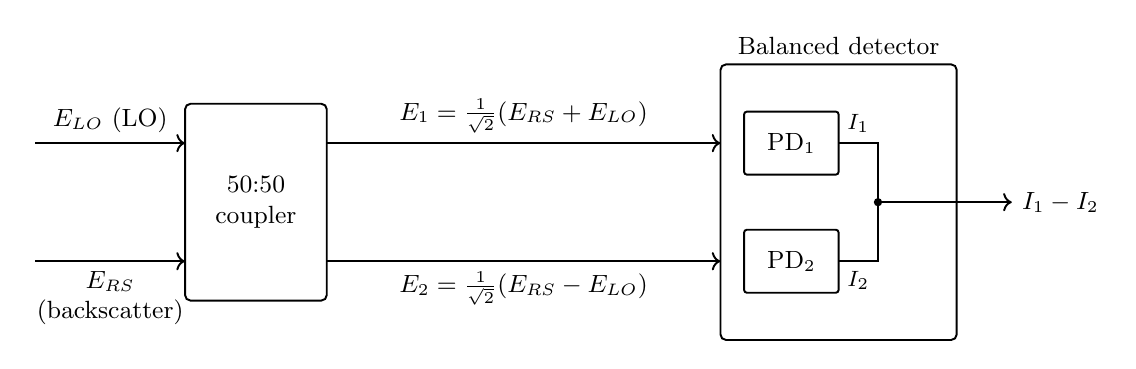
\begin{tikzpicture}[font=\small, line width=0.7pt]

% ---- inputs ----
\draw[->] (0.3,2.25) -- (2.2,2.25);
\node[above] at (1.25,2.25) {$E_{LO}$ (LO)};
\draw[->] (0.3,0.75) -- (2.2,0.75);
\node[below, align=center] at (1.25,0.75) {$E_{RS}$\\(backscatter)};

% ---- coupler ----
\draw[rounded corners=2pt] (2.2,0.25) rectangle (4.0,2.75);
\node[align=center] at (3.1,1.5) {50:50\\coupler};

% ---- coupler outputs ----
\draw[->] (4.0,2.25) -- (9.0,2.25);
\node[above] at (6.5,2.25) {$E_1 = \tfrac{1}{\sqrt{2}}(E_{RS} + E_{LO})$};
\draw[->] (4.0,0.75) -- (9.0,0.75);
\node[below] at (6.5,0.75) {$E_2 = \tfrac{1}{\sqrt{2}}(E_{RS} - E_{LO})$};

% ---- balanced detector ----
\draw[rounded corners=2pt] (9.0,-0.25) rectangle (12.0,3.25);
\node[above] at (10.5,3.25) {Balanced detector};
\draw[rounded corners=1pt] (9.3,1.85) rectangle (10.5,2.65);
\node at (9.9,2.25) {PD$_1$};
\draw[rounded corners=1pt] (9.3,0.35) rectangle (10.5,1.15);
\node at (9.9,0.75) {PD$_2$};

% ---- difference ----
\draw (10.5,2.25) -- (11.0,2.25) -- (11.0,0.75) -- (10.5,0.75);
\node[above, font=\footnotesize] at (10.75,2.25) {$I_1$};
\node[below, font=\footnotesize] at (10.75,0.75) {$I_2$};
\fill (11.0,1.5) circle (1.5pt);
\draw (11.0,1.5) -- (12.0,1.5);

% ---- output ----
\draw[->] (12.0,1.5) -- (12.7,1.5);
\node[right] at (12.7,1.5) {$I_1 - I_2$};
\end{tikzpicture}
\caption{Balanced detection. The 50:50 coupler delivers the sum and difference
of the backscatter and LO fields to two matched photodiodes; the output is the
difference of their photocurrents, in which the common-mode terms cancel and
only the beat term $2\sqrt{P_{LO} P_{RS}}\cos(2\pi\Delta f t)$ remains.}
\label{fig:balanceddetector}
\end{figure}

It can thus be seen that balanced detection provides the advantage of cancelling RIN. This allows for the final detected signal to theoretically be able to achieve the desired shot-noise limited operation (if other sources of noise are also eliminated). 

\subsection{Transmit and Receive Optics: Monostatic vs Bistatic}
    For a DWL system there are two optical configurations which are commonly used - bistatic and monostatic. This section discusses the differences between the two.

    \subsubsection{Bistatic}
    Bistatic configurations use one lens to emit the laser into the atmosphere, and another to receive the backscatter signal. One distinct advantage of a bistatic configuration, is that back reflections of the beam from the lens used for emission are not coupled into the mixed signal, and thus do not appear at the detector \cite{cariou2006laser}. This serves to reduce phase induced intensity noise (discussed in \autoref{sec:lit-linewidth}. However, this is at the cost of greatly increased complexity, due to additional considerations of alignment of the two lens apertures \cite{harris_role_1998} \cite{bennett_doppler_2003}. 
    
    \subsubsection{Monostatic}
    A monostatic configuration uses a single lens aperture for both the emission of the laser, and the receiving of the backscatter signal. A fiber optic circulator can then be used to ensure the emitted signal and the received signal do not interfere, and are routed appropriately in the system. This has the distinct advantage of not requiring any additional lenses, and alignment considerations, and indeed has become the norm for such systems due to this reduced complexity \cite{hill_remote_nodate}.  
        

    \subsection{Ranging: Pulsed versus Continuous Wave}
    % Range gating vs. focus-defined probe volume.
    % Pulse length / minimum range and dead-time constraints.
    % Close by justifying CW on physics grounds at the ranges of interest.
    Coherent DWL systems have two distinct methodologies which can be applied in order to determine at what distance from the system a measured wind-speed is occurring. The methodology differs depending on a key architectural choice of the system, namely whether the LiDAR beam is on for longer periods of time - known as continuous wave (CW) - or if it is pulsed. Both of these architectures hold their own advantages and disadvantages, which will be discussed in this section.

    \subsubsection{Pulsed LiDAR}
    As the name suggests, a pulsed LiDAR system emits its beam in a short pulse. Depending on the pulse duration, a given volume of air - called the probe volume - will be illuminated at an instant of time, and will create backscatter. This volume naturally moves through the air as the beam propagates radially. Thus, by using extremely precise timing on the returned backscatter, it can be determined which distance "slice" of air that backscatter was generated by, and thus, what the wind-speed for that particular "slice" is. The wind-speed for that distance is averaged over the probe volume, thus a shorter pulse will give greater spatial accuracy due to its shorter probe volume. This technique is known as range-gating, and has been widely applied in commercial and scientific DWL systems. \cite{cariou_leosphere_nodate} \cite{wagner_power_2014} \cite{letizia_characterization_2023}. A distinct advantage of range-gating is that the probe volume remains the same at all distances, including longer ones, giving it constant range resolution for longer distances than CW systems \cite{cariou_leosphere_nodate} (described below). However, it must also be noted that typical pulsed systems are ineffective in ranges below tens of metres, because the pulse length is at least as long as the desired range \cite{hill_remote_nodate}. 

    \subsubsection{Continuous-Wave LiDAR}
    Continuous-wave systems emit a continuous beam through the atmosphere. This simplifies the design cost and complexity of the systems \cite{cariou_leosphere_nodate} \cite{hill_remote_nodate}, and no precise pulse timing or receive timing is required. CW systems achieve ranging by using optics to focus the beam at a specific distance. This gives a Lorentzian spatial weighting function along the beam length, with a peak at the focus point of the beam (the point with highest intensity), thus concentrating the detection sensitivity around the focus, at the expense of contributions from other ranges. However, the effective probe volume varies \textbf{quartically} with the distance of the focal point from the source, thus significantly increasing the volume over which the Doppler shift (and therefore wind-speed) is averaged at longer focal distances. Therefore for longer ranges, spatial resolution severely decreases, and it is not possible to gate the measurements for any specific region of air before the focal point. For this reason, CW systems are not well-suited for long ranges of several hundred meters \cite{hill_remote_nodate}, however at short ranges they can be more effective than pulsed systems, owing to the previously mentioned limitations of pulsed systems, relating to pulse length. 

    
    

% ---------------------------------------------------------------------


    
    
   
        
\chapter{System Design}

\section{Introduction}
This chapter details the design of a Doppler wind LiDAR system. As discussed in the introduction and scope of this report, the system is a benchtop prototype whose purpose is to make the sensitivity of a DWL measurable and attributable to specific component and architecture choices. As such, the primary considerations will be noise-levels, sensitivity, and the overarching principles of physics governing DWL systems. This system design will thus not include the design of housing for field deployment, nor will it be concerned with real-time post-processing pipelines for the system's data (which would be required in a field-deployed system). Furthermore, several key components that would be typical in a scientific- or industry-grade, field-deployable DWL system are deliberately omitted in order to reduce costs, at little functional expense for a benchtop system. Where possible, the system was made extensible for future iterations and field deployment.

First \autoref{sec:design-sysArch} gives an overview of the architecture chosen, as synthesised from the various architecture types reviewed in \autoref{sec:litReview}, and with respect to the project's overarching goals. Thereafter, \autoref{sec:design-sysReqs} discusses the functional and performance requirements of the system. Finally, section \ref{sec:design-ComponentChoices} details the specific components chosen to meet these requirements. 

\section{System Architecture}
\label{sec:design-sysArch}
From the reviewed literature in \autoref{sec:litReview}, it was decided that an \textbf{all-fibre, coherent detection, continuous-wave, monostatic} DWL system with \textbf{balanced detection} would be built, with sampling and digitisation to be handled by a benchtop oscilloscope, and post-processing done on a laptop computer. This section details why these architectural choices were made, using summarised information from \autoref{sec:litReview} with respect to the project goals, and discusses any significant implications for the system. 

\subsection{Coherent detection}
\label{sec:design-sysArch}
The direct detection technique requires the
Rayleigh/Mie scattering ratio and temperature, an absolutely stabilised laser, etalon
control to 1 milli-Kelvin, and very precise physical alignment and calibration
\cite{korb_theory_1998,colberg_diode-laser-based_2026,werner_doppler_2005}. These present substantial challenges to an undergraduate project, particularly the stabilised laser and etalon temperature control. The one advantage which direct detection holds, which is the capability of using molecular backscatter when aerosol backscatter is not available, is irrelevant in an aerosol-rich controlled lab environment, which is the only environment this system will be tested in.

By contrast, coherent detection is far more common in the literature, and thus has more practical information and sources for components. Furthermore, mixing with the LO also permits shot-noise-limited operation through the effective amplification of the return signal, and rejects unwanted light not
mode-matched to the LO \cite{hill_remote_nodate} (e.g. other LiDAR systems, or the sun), thus reducing sources of potential interference. The architecture thus lends itself to a more elegant, direct method of measuring the Doppler shift, via optical mixing and subsequent detection. 

For these reasons, a coherent detection system was chosen for this project build. 

\subsection{Homodyne mixing}
Homodyne mixing places the Doppler shift at baseband with no additional frequency shift, and no additional components necessary, whereas heterodyne operation requires an acousto-optic
modulator (AOM) in the LO or transmit arm
\cite{harris_role_1998,abdelazim_development_2015}. The tradeoff  is the sign ambiguity as discussed in \autoref{sec:lit-homohetero}, where only the velocity \textbf{magnitude} is
measured in a homodyne system, whereas a heterodyne system can resolve the direction.

For a benchtop-scale system which primarily aims to present the working principles of a DWL system and a sensitivity analysis, and where the direction of the flow being measured will always be known, it is not necessary to recover signed velocity. Adding an AOM thus adds needless complexity, and adds an additional unnecessary cost to a budget-constrained project. Crucially however, the addition of an AOM for a future iteration of the system is simple, and does not require the redesign of any parts of the current system. For these reasons it was thus decided to omit the AOM, and to therefore construct a \textbf{homodyne} coherent detection system.

\subsection{Balanced detection}
As discussed in \autoref{sec:lit-BalancedDetection}, balanced detection holds the advantage of providing a 3dB improvement in SNR (in shot-noise limited operation) as compared to single ended detection. It also allows RIN to be largely cancelled, further allowing SNR improvement, and allowing the system to better approach the shot-noise limit (see Appendix \ref{appendix:RIN}). For these reasons, it was decided that a balanced detection setup would be used.

\subsection{Monostatic optics}
For this project, it was decided to use a monostatic optical configuration - where a single aperture serves both transmit and receive, separated by a fibre
circulator, with no second lens and no alignment of two lenses necessary. A bistatic arrangement would
keep transmit-optics back-reflections away from the detector, at the cost of greatly increased alignment complexity
\cite{cariou2006laser,harris_role_1998,bennett_doppler_2003}, as well as the additional cost of 2 sets of optics, and equipment needed for alignment. The accepted
tradeoff here is thus that back-reflections from the transmit path reach the detector and
raise the noise floor through PIIN (see \autoref{sec:lit-linewidth}).

\subsection{Continuous-wave operation}
Pulsed systems are ineffective below tens of metres because the pulse length is typically at least as long as this range \cite{hill_remote_nodate}. a CW system needs no pulse or receive timing, which simplifies design and can reduce costs (due to lower component count). It is also the more effective of the two at short range. One of the significant performance costs of a CW system however is reduced spatial resolution, particularly at long ranges, as spatial resolution is defined by focus rather than gating with timing (see \autoref{sec:lit-pulsedCW}). Seeing as a benchtop system requires operation at short ranges in the order of tens of centimeters to one or two meters, a CW system will be best suited here due to its simplicity, and its advantages at short range, as well as the irrelevance of long-range limitations.

\subsection{All-fibre construction}
For this project it was decided that an all-fibre construction would be used - meaning that fibre optic cables would be used to transmit the LO and emission beams, and return signals, rather than transmitting the beams through free-space. Single-mode fibre makes the mode-matching between LO and return that coherent detection requires automatic, removes free-space alignment complexities, and gives access
to widely and cheaply available telecom components
\cite{bennett_doppler_2003,abari_all-fiber_2014,abdelazim_development_2015}. Non polarisation-maintaining fibre is used, owing to cost considerations as compared to polarisation-maintaining fibre.
The accepted tradeoff of standard (non-polarisation-maintaining) fibre is that the polarisation of LO and return is not fixed, which will reduce the heterodyne efficiency of the system, and thus reduce the measureable Doppler peak \cite{cariou2006laser}. 


\subsection{System Architecture Diagram}
\autoref{fig:design-architecture} below shows a functional block-diagram of the system's decided-upon architecture. In this diagram, the signal path can clearly be seen from laser source, through the splitter (splitting into LO and transmit beam). Thereafter the transmit beam gets routed via port 1 --\textgreater 2 of the circulator to the monostatic optics, which also receives the backscatter signal to be routed via port 2 --\textgreater 3 of the circulator. The local oscillator and backscatter signals are mixed in the optical mixer, and then detected by a balanced photodetector, from which the final output beat signal can be sampled and processed. 
\begin{figure}[H]
\centering
\resizebox{\textwidth}{!}{%
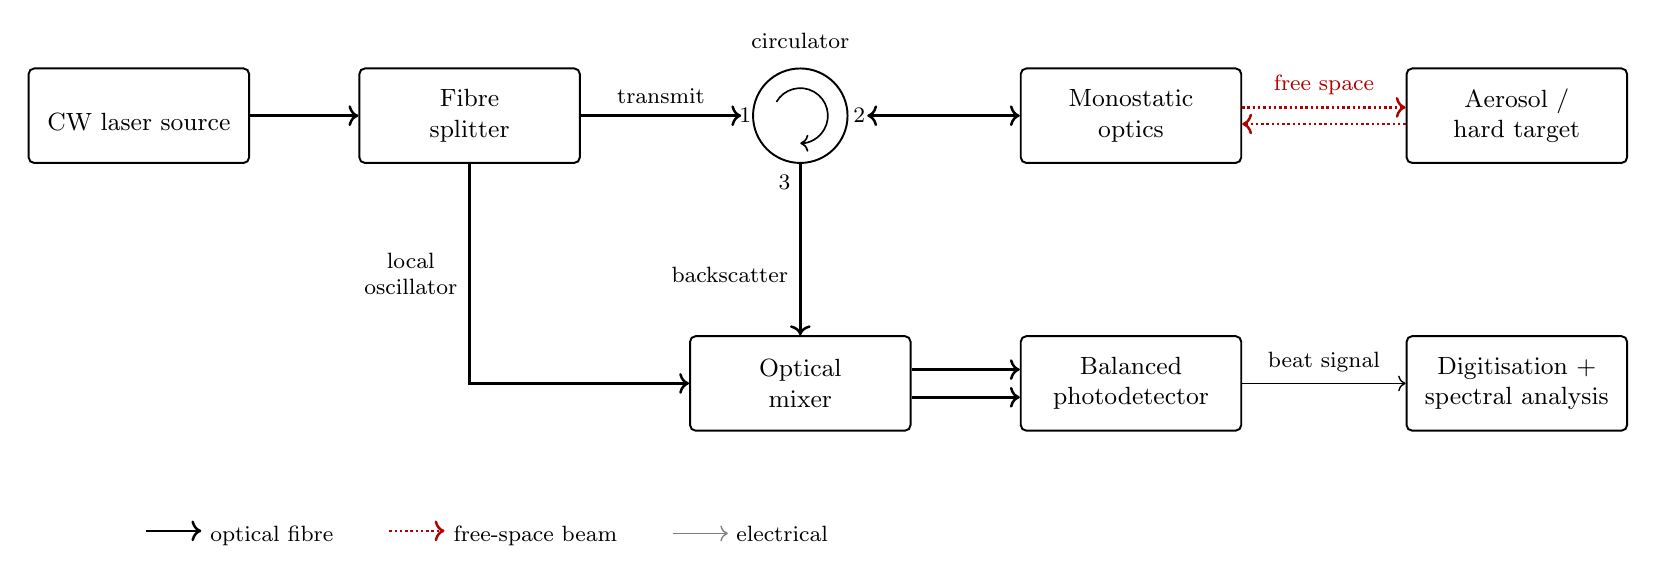
\begin{tikzpicture}[
  font=\small, line width=0.7pt,
  block/.style={draw, rounded corners=2pt, align=center, minimum height=1.2cm,
                minimum width=2.8cm, inner sep=5pt},
  fibre/.style={->, line width=0.9pt},
  fibreBoth/.style={<->, line width=0.9pt},
  free/.style={->, line width=0.9pt, red!70!black, densely dotted},
  elec/.style={->, line width=0.5pt, gray},
  leak/.style={->, line width=0.7pt, red!70!black, dashed},
  lbl/.style={font=\footnotesize, align=center, inner sep=2pt}
]

% ---- top row ----
\node[block] (laser) at (0,0)  {\\CW laser source};
\node[block] (cpl)   at (4.2,0) {Fibre\\splitter};
\node[draw, circle, minimum size=1.2cm] (circ) at (8.4,0) {};
\draw[->, line width=0.6pt] (8.4,0) ++(150:0.35) arc (150:-90:0.35);
\node[lbl] at (7.7,0)    {1};
\node[lbl] at (9.15,0)    {2};
\node[lbl] at (8.2,-0.85) {3};
\node[lbl] at (8.4,0.95)  {circulator};
\node[block] (coll)  at (12.6,0) {Monostatic\\optics};
\node[block] (tgt)   at (17.5,0) {Aerosol /\\hard target};

\draw[fibre] (laser.east) -- (cpl.west);
\draw[fibre] (cpl.east)   -- (7.65, 0) node[midway, above=2pt, lbl] {transmit};
\draw[fibreBoth] (9.25, 0)  -- (coll.west);
\draw[free] ([yshift= 3pt]coll.east) -- ([yshift= 3pt]tgt.west)
  node[midway, above=2pt, lbl] {free space};
\draw[free] ([yshift=-3pt]tgt.west)  -- ([yshift=-3pt]coll.east);

% ---- bottom row ----
\node[block] (comb) at (8.4,-3.4)  {Optical\\mixer};
\node[block] (det)  at (12.6,-3.4) {Balanced\\photodetector};
\node[block] (dsp)  at (17.5,-3.4) {Digitisation +\\spectral analysis};

\draw[fibre] (cpl.south) |- (comb.west)
  node[pos=0.25, left=2pt, lbl] {local\\oscillator};
\draw[fibre] (circ.south) -- (comb.north)
  node[pos=0.65, left=2pt, lbl] {backscatter};
\draw[fibre] ([yshift= 5pt]comb.east) -- ([yshift= 5pt]det.west);
\draw[fibre] ([yshift=-5pt]comb.east) -- ([yshift=-5pt]det.west);
\draw[elec, black] (det.east) -- (dsp.west) node[midway, above=2pt, lbl] {beat signal};

% ---- legend ----
\node[lbl, anchor=west] at (0,-5.3) {%
  \tikz\draw[->, line width=0.9pt] (0,0)--(0.7,0); optical fibre \qquad
  
  \tikz\draw[->, line width=0.9pt, red!70!black, densely dotted] (0,0)--(0.7,0); free-space beam \qquad
  
  \tikz\draw[->, line width=0.5pt, gray] (0,0)--(0.7,0); electrical};
\end{tikzpicture}}
\caption{Block diagram of the chosen architecture: all-fibre, coherent,
continuous-wave, monostatic, homodyne, with balanced detection}
\label{fig:design-architecture}
\end{figure}

\section{System Requirements Analysis}
\label{sec:design-sysReqs}
Now that a system architecture has been decided on, requirements which are specific to this choice of architecture, and which are related to the project goals can be synthesised. The requirements for the system are divided into two sets: functional requirements, which define the ideal outcomes which are desired from the system, and performance requirements, which define specific metrics which are to be measured and quantified with respect to the goals of the functional requirements. 

\subsection{Functional requirements}
\begin{enumerate}

  \item Measure the line-of-sight velocity of a target from the          Doppler shift of coherently detected backscatter,
        using a monostatic all-fibre homodyne architecture with balanced detection and continuous-wave operation.
  \item Operate on both a diffuse hard target of known velocity and on air seeded with smoke or fog. 
  \item Produce a velocity estimate from a recorded spectrum using a stated, reproducible detection criterion (threshold relative to the system's noise floor).
\end{enumerate}

\subsection{Performance requirements}
From the desired functional requirements, a set of performance requirements can be synthesised; these are given in \autoref{tab:requirements} below along with the IDs of the tests which will verify them. 

%It must be noted again here that this project's goals chiefly concern the measurement and characterisation of noise and SNR in a constrained DWL system build, and how these aspects relate to component choice. As such, the majority of these requirements are concerned with the characterisation of the system relative to an ideal system, and thus the quantification of the system's limitations - rather than attempting to achieve performance specifications which will allow all the functional requirements to be met. 
\begin{table}[H]
\centering
\small
\begin{tabular}{|p{0.5cm}|p{3cm}|p{9cm}|p{1.7cm}|}
\hline
\textbf{ID} & \textbf{Requirement} & \textbf{Value} & \textbf{Verified by} \\ \hline
P2 & Detector noise & approaching ideal shot-noise-limited behaviour: total
     detector noise (electronic noise + residual RIN after balanced
     detection) within \SI{1}{\decibel} of the shot-noise limit
    & A1, A2 \\ \hline
 P4 & Phase-induced intensity noise (PIIN) & Level (in dB) and spectral shape measured;
 agreement with the path-mismatch model of \cite{harris_role_1998}
    within \SI{6}{\decibel} & B \\ \hline
P3 & Total system noise & Total noise floor (shot + electronic + residual RIN + PIIN) quantified with respect to the shot-noise limit, and sources of excess noise described and characterised & B \\ \hline
 P1 & Velocity detection on a hard target & Doppler peak detected at $ \gg 5\times\sigma$ (5 times the noise standard deviation) above the  mean, at $N \leq 1000$ averages, for a hard target 10cm away from laser emission & C \\ \hline
P5 & Low-velocity limit & Minimum resolvable LOS speed of $\leq$ \SI{0.1}{\metre\per\second} on a hard target & C \\ \hline
P6 & Detection of wind-speed in seeded air (smoke or fog) & Doppler peak detected at $ \gg 5\times\sigma$ (5 times the noise standard deviation) above the  mean, at $N \leq 10 000$ averages 
& D \\ \hline
P7 & Velocity accuracy & Doppler velocity within 5\% of ground-truth velocity of target (hard target and seeded flow) & C, D \\
\hline
\end{tabular}
\caption{Performance requirements and their verification tests.}
\label{tab:requirements}
\end{table}

\section{Component Choices}
\label{sec:design-ComponentChoices}
This section details the specific component selections which were made for the system. These selections were made to best suit the functional and performance requirements of the system. It must be noted that this project is constrained when compared to typical scientific or industrial DWL systems. As such, many component choices were driven by cost, availability, and time-frame considerations, rather than simply their suitability for the system. This is however a suitable approach for the goals of the project, which are to illustrate the principles and physics involved in a DWL system, and to quantify system performance with respect to component choices. 
\subsection{Laser Source}
    The selection of an appropriate laser source is critical to ensure good performance of a DWL system. There are numerous properties of a laser source which should be considered, and which will be detailed in this section. After discussion on these properties, a suitable laser source is selected. 

    \subsubsection{Wavelength}
    There are many suitable wavelengths for DWL systems, as detailed by Cariou et. al \cite{cariou2006laser}. There is much discussion around SNR optimisation and backscatter maximisation for varying wavelengths \cite{bennett_doppler_2003}, however owing largely to practical advantages, a wavelength of 1550nm has emerged as a common choice for both commercial and scientific DWL systems \cite{abari_all-fiber_2014}. Fiber optics telecommunications  commonly operate at this wavelength - thus making components designed for this wavelength readily commercially available and significantly cheaper than alternatives \cite{cariou2006laser}, \cite{abdelazim_development_2015}, \cite{hill_remote_nodate}. Additionally, laser beams at 1550nm are eye-safe at significantly higher power levels (up to multiple Watts), compared to shorter wavelengths \cite{cariou2006laser}, reducing safety concerns. For this reason it was decided that a 1550nm laser source would be used for this project. 
    
    \subsubsection{Power Level}
    % EDFAs
    % Backscatter intensity 
    As previously discussed, the ability of a DWL system to measure wind-speed depends on the measurement of aerosol backscatter of the emitted beam. 
    
    The time-averaged power of the backscatter signal into a receiver can be expressed as \cite{hill_remote_nodate}:
    
        \begin{equation}
            P_s = \pi P_t \beta(\pi) \lambda
            \label{eqn:backscatterPower}
        \end{equation}

    Where $P_s$ is the time averaged backscatter signal power, $\beta(\pi)$ is the atmospheric scattering coefficient (evaluated at $\pi$, i.e. scattering at $\pi$ radians, back towards the source), and $\lambda$ is the wavelength of the transmitted light. Note that $\beta(\pi)$ also holds a wavelength dependence, and thus $P_s$ does not necessarily scale linearly with increasing wavelength, as the equation may suggest, but instead resolves to a near cancellation of the wavelength dependence between some frequency ranges \cite{bennett_doppler_2003}.
    
    It can be seen in \autoref{eqn:backscatterPower} that there is a linear dependence on $P_t$, the power of the transmitted beam. Thus, a higher-powered transmit laser source would give a larger return signal to be measured, increasing the sensitivity of the system by increasing the SNR of the system \cite{bennett_doppler_2003}. 

    A setup commonly used to achieve higher emitted laser power here is the master-oscillator power-amplifier (MOPA) configuration \cite{cariou2006laser}, \cite{bennett_doppler_2003}. This separates the functions of the laser source - allowing for a low-power, highly coherent, narrow linewidth laser source to be used as a master-oscillator and an amplifier to increase the power levels of the master oscillator beam, while maintaining its spectral purity. This also allows the local oscillator to be derived from the master oscillator, eliminating the need to have two separate laser sources - one for LO, one for output - which would need to have a stable frequency relationship \cite{cariou2006laser}, something which requires careful design to achieve, as illustrated by Colberg et al. \cite{colberg_diode-laser-based_2026}.  

    As noted by Bennett, such power amplifiers (commonly Erbium-doped fiber amplifiers; EDFAs) make up a significant portion of the cost of a DWL system. Indeed, more than 20 years after the writing of Bennett's paper, the cost of EDFAs remain prohibitively expensive for a project at this scale. For EDFA systems which are able to amplify signals to hundreds of milli-Watts or multiple Watts (which is a typical power level for such a system \cite{abdelazim_development_2015}\cite{cariou_leosphere_nodate}\cite{cariou2006laser}), current prices range in the thousands to tens of thousands of USD (see Appendix). 
    
     For this reason, the use of a power amplifier for the laser source is disqualified for this project on the grounds of cost. The system was however designed such that the addition of such an amplifier would be possible at a later stage.
     
     Due to the relatively low powers available for laser sources without power amplification (in the tens of milli-Watts), other avenues to improve detection sensitivity will be required. Bennett identifies another option for increasing the sensitivity of a DWL system - which is to average over many returns \cite{bennett_doppler_2003}. This is the approach which will be taken for this project. Additionally, owing to this constraint in laser source power, all tests which concern wind-speed measurement in air will be performed using air seeded with smoke and/or fog. This will increase backscatter levels by increasing $\beta(\pi)$ in \autoref{eqn:backscatterPower}, and thus reduces the need for the power amplifier for this benchtop-scale system. The level of seeding required for a lower-power laser source to detect wind-speed is one of the investigations of this project.

    \subsubsection{Linewidth}
    \label{sec:lit-linewidth}
    Linewidth can be seen as a measure of the spectral purity of a laser source, and is one of the most critical parameters in the design of a DWL system. A narrow linewidth is highly desirable for DWL applications, as this will significantly reduce the phase-induced intensity noise (PIIN) in a DWL system, and allow the system to therefore have a better SNR and sensitivity to detect small backscatter signals. Furthermore, the linewidth of a laser source has a significant effect on how broad the returned backscatter signal's Doppler shifted peak is, particularly at longer ranges. This will result in the system having worse precision, and not being able to resolve turbulence in the air as well. For a full discussion on the mathematical and physical meaning of linewidth, as well as a treatment on how linewidth affects PIIN and the broadened peak, see Appendix \ref{appendix:PIIN}. Cariou et al. make the claim that linewidths typical of DFB diodes (0.5 - 5MHz, see \autoref{tab:design-laser-sources}) disqualify them for use in CW DWL systems due to their PIIN, however, Bennett shows that indeed a DFB source with a linewidth of 1.4MHz can be used for these purposes, provided careful attention is given to other design considerations, such as optical fiber path length matching \cite{bennett_doppler_2003}. The analysis of noise in the system, and the associated constraints arising from the use of a comparatively wider linewidth laser source indeed forms a key part of this project, owing to budget considerations, as will be discussed below and in \autoref{sec:noiseAnalysis}.
    
    

    \subsubsection{Laser source types and selection}
    There are many types of laser sources available on the market. In the selection of a laser source for this project, the primary driver was cost and availability, with the design goals being to maximise power level and minimise linewidth, while fixing the wavelength at 1550nm. After selecting the best available laser source for these parameters, the performance of the laser source will then be analysed, and recommendations based on its properties and performance can then be made. 

\begin{table}[H]
\centering\small
\renewcommand{\arraystretch}{1.2}
\begin{tabular}{@{}|p{2.6cm}|p{1.9cm}|p{1.7cm}|p{6.0cm}|p{2.2cm}|@{}}
\hline
\textbf{Source type} & \textbf{Linewidth (typ.)} & \textbf{Power, unamplified} & \textbf{Noise and practical notes} & \textbf{Indicative cost (USD)} \\
\hline
Fabry--P\'erot laser diode &
multi-mode; not single-frequency &
\SIrange{10}{100}{\milli\watt} &
Multi-mode, Unsuitable for coherent detection due to this. \cite{harris_role_1998}.  &
$<100$ \\
\hline
DFB laser diode &
\SIrange{0.5}{5}{\mega\hertz} &
\SIrange{10}{40}{\milli\watt} &
Relaxation peak \SI{\sim1}{\giga\hertz}, far above the Doppler band, thus is RIN flat and low in the frequency band of interest \cite{cariou2006laser}. Needs external driver and temperature controller. &
\numrange{100}{1000} (module) \\
\hline
Planar external-cavity semiconductor &
$<1$ to \SI{15}{\kilo\hertz} &
\SIrange{10}{30}{\milli\watt} &
Integrated driver, marketed for wind lidar.&
quote only; low thousands \\
\hline
Er-doped DFB fibre laser &
$<0.1$ to \SI{10}{\kilo\hertz} \cite{harris_role_1998} &
\SIrange{10}{40}{\milli\watt} &
Common source of choice for CW anemometry due to narrow linewidth \cite{cariou2006laser,hill_remote_nodate, abdelazim_development_2015}. Relaxation peak near \SI{1}{\mega\hertz}, so higher RIN in the frequency band of interest \cite{cariou2006laser}. &
quote only; tens of thousands \\
\hline
\end{tabular}
\caption{Laser source classes at \SI{1550}{\nano\metre}. Linewidths and powers are typical of commercial devices; approximate costs are as of September 2026 and exclude drivers, controllers and import costs.}
\label{tab:design-laser-sources}
\end{table}

From these available laser source options, it was decided that a DFB laser diode would be used. While the wider linewidth, as compared to Planar external-cavity semiconductor diodes or Er-doped DFB fibre lasers is likely to substantially increase PIIN, measures such as fiber length matching will be investigated to reduce PIIN for lower-range, tabletop operation (see \autoref{sec:testingPIIN}), and these narrow linewidth sources are out of budget for this project. 

The final specifications of the obtained laser diode are as follows:
\begin{table}[H]
	\centering
	\label{tab:dfb-laser}
	\begin{tabular}{@{}ll@{}}
		\toprule
		\textbf{Parameter} & \textbf{Value} \\
		\midrule
		Wavelength                  & 1550~nm \\
		Rated output power          & 20~mW \\
		Linewidth                   & 2~MHz \\
		Operating current at 20mW & 58~mA \\
		Fibre output                & Single-mode, FC/APC \\
		\bottomrule
	\end{tabular}
	\caption{Key properties of the selected DFB laser diode
		(BFLD-1550-20SM-FA2). Full specifications are given in
		\autoref{appendix:laser}.}
\end{table}

\subsection{Laser driver and temperature control}
In order to keep the laser diode at a constant operating point, a constant current source must be used to drive it, and a temperature controller should be used. Temperature and current fluctuations present in the laser output as fluctuations in wavelength and output power \cite{Gwinner2024}, which can have a significant effect on the noise in measurements, particularly in a sensing system, such as a DWL, for which measurements of very small signals is required.

 Perhaps the greater consideration however is the safety of the laser diode. The laser diode chosen forms the single biggest expense in this DWL system, and thus protecting it is of vital importance to this project. Laser diodes are extremely sensitive to transients and overvoltage events, which can easily damage them \cite{Gwinner2024}. Circuitry for these ends may be custom-designed and manufactured as a PCB, however, this is a complex process, and is best-suited to systems where commercially available driver and temperature control circuitry is unsuitable. Thus, for this project it was decided that off-the-shelf circuitry would be used for these ends, so that the expensive laser diode is safeguarded against possible custom design flaws or oversights of a first-time designer. Commercial off-the-shelf units integrate soft-start circuitry, current control, current monitoring, protection against overvoltage and overcurrent events and transients into a single package.
 
 The Koheron DRV200S-A-200 laser driver was chosen, due to its very low noise characteristics, and the suitability of the current range and limit for the BFLD-1550-20SM-FA2 laser diode chosen above. The Koheron TEC100L-50 temperature controller was chosen from the same supplier, and has an adequate setpoint range and stability for the project. The respective specifications of the selected laser driver and  temperature controller are given below:
 
 \begin{table}[H]
 	\centering
 	\begin{minipage}[t]{0.48\textwidth}
 		\centering
 		\label{tab:drv200s}
 		\begin{tabular}{@{}ll@{}}
 			\toprule
 			\textbf{Parameter} & \textbf{Value} \\
 			\midrule
 			Current range             & 0--200~mA \\
 			Current limit (adj.)      & 65--300~mA \\
 			Noise density (1~kHz)     & 270~pA/$\sqrt{\text{Hz}}$ \\
 			RMS noise (10~Hz--1~MHz)  & 265~nA \\
 			Temperature coefficient   & 30~ppm/$^\circ$C \\
 			\bottomrule
 		\end{tabular}
 		\caption{Key specifications of the Koheron DRV200S-A-200
 			laser diode driver.}
 	\end{minipage}
 	\hfill
 	\begin{minipage}[t]{0.48\textwidth}
 		\centering
 		\label{tab:tec100l}
 		\begin{tabular}{@{}ll@{}}
 			\toprule
 			\textbf{Parameter} & \textbf{Value} \\
 			\midrule
 			TEC current               & $\pm$1.15~A \\
 			Setpoint range            & 10--40~$^\circ$C \\
 			24~h stability            & 0.005~$^\circ$C \\
 			Temperature coefficient   & 0.002~$^\circ$C/$^\circ$C \\
 			Supply voltage            & 5~V \\
 			\bottomrule
 		\end{tabular}
 		\caption{Key specifications of the Koheron TEC100L-50
 			temperature controller.}
 	\end{minipage}
 \end{table}
 
 \subsection{Detector}
 Balanced detectors typically include two matched photodiodes, connected differentially to a low-noise transimpedance amplifier which converts the photodiode current into a measurable voltage. Seeing as the beat signal which will be measured is in the order of mega-Hertz in frequency, much care needs to be taken when designing the electronic circuitry of the detector to avoid parasitic effects, such as stray capacitance and inductance, which can cause amplifier instability and limit bandwidth, as well as susceptibility to electromagnetic interference. Given the difficulty of proper RF design, to simultaneously achieve high bandwidth, low noise and high common-mode rejection in a custom design, a commercial balanced detector was selected so that project effort could be focused on the lidar system itself.
 
 The Koheron PD100B Balanced Photodetector was selected for use in this project, with the key specifications given in \autoref{tab:pd100b} below:
 
 \begin{table}[H]
 	\centering
 	\label{tab:pd100b}
 	\begin{tabular}{@{}ll@{}}
 		\toprule
 		\textbf{Parameter} & \textbf{Value} \\
 		\midrule
 		Photodiode responsivity       & 0.9~A/W \\
 		Max.\ input power (per diode) & 1.5~mW \\
 		Bandwidth ($-3$~dB)           & 160~Hz--100~MHz \\
 		Transimpedance gain           & 39~kV/A \\
 		Input current noise density   & 8~pA/$\sqrt{\text{Hz}}$ \\
 		CMRR (1~MHz)                  & 35~dB \\
 		\bottomrule
 	\end{tabular}
 	\caption{Key specifications of the Koheron PD100B-AC balanced photodetector.
 		Full specifications are given in \autoref{appendix:pd100b}.}
 \end{table}
 
 The photodetector has a bandwidth of 160Hz - 100MHz, thus DC photocurrent is blocked (this is desired, seeing as the measured quantity of interest is the frequency power at MHz-range frequencies). This will also allow signals of up to 100MHz to be effectively detected. A beat frequency of 100MHz corresponds to a wind-speed of approximately 129m/s (464km/h), which is clearly far above any wind-speed which the system would reasonably need to detect. It can also be seen that the detector has a very low electronic noise floor of 8pA/$\sqrt{Hz}$, which can easily be swamped out by the shot-noise from the LO to achieve shot-noise limited behaviour, and the CMRR is high, allowing RIN to be very effectively cancelled. 
 
 \subsection{Fiber Optics}
 \subsubsection{Optical Mixer, Circulator}
A standard 50:50 non-polarisation maintaining FC/APC connector type fiber optic coupler is to be used as the optical mixer (see \autoref{fig:design-architecture}). This has two input signals which are mixed at a 50:50 ratio, and split into two output signals for balanced detection.

 A standard 3-port non-polarisation maintaining FC/APC fiber optic circulator is obtained to allow transmission and reception of signals from the same optics. 
\subsubsection{Fiber Splitter}
 More care must be taken in selecting the fiber splitter, as the ratio here determines how much of the laser source power is directed towards emission, and how much towards use as a local oscillator for down-stream mixing.
 
  As discussed in \autoref{sec:litReview}, the LO power has a significant effect on the noise characteristics and the performance of the system. While the LO power can be indirectly varied by varying the laser source power (via current), this will also vary the transmit power. Thus, a splitter ratio should be selected which allows for a suitable LO power level which allows for shot-noise limited operation, when the laser is set to an output power level which provides sufficient transmit power. 
 
 The lower bound on the LO power is set by the requirement for shot-noise-limited
 operation, which occurs when the LO shot noise exceeds the 
 electronic noise of the detector (see \autoref{sec:lit-noiseSources}). For the
 balanced detector, the shot noise current density is
 $I_{\text{sn}} = \sqrt{2qR P_{\text{LO}}}$ (derived from Kikuchi et al. \cite{kikuchi_fundamentals_2016}), where R is the photodetector's responsivity, and q is the charge of an electron, so equating this to the PD100B input
 noise density $I_n = 8~\text{pA}/\sqrt{\text{Hz}}$ gives
 \begin{equation}
 	P_{\text{LO,min}} = \frac{i_n^2}{2qR}
 	= \frac{(8\times10^{-12})^2}{2(1.602\times10^{-19})(0.9)}
 	\approx 222~\mu\text{W}.
 	\label{eq:PLOmin}
 \end{equation}
 The upper bound is set by photodiode saturation. The 50:50 coupler divides the
 LO equally between the two photodiodes, which are each rated to a maximum of 1.5~mW, so
 $P_{\text{LO,max}} \approx 3$~mW.
 
 For a splitter that directs a fraction $\kappa$ of the laser power $P_L$ to the
 LO, the condition $P_{\text{LO,min}} \leq \kappa P_L \leq P_{\text{LO,max}}$ defines
 the range of usable laser powers. With $\kappa = 0.1$, this gives
 $2.2~\text{mW} \leq P_L \leq 30~\text{mW}$, which spans the full output range of
 the 20~mW source. At full power, this yields an LO of 2~mW, approximately
 $9\times$ (9.5~dB) above the electronic noise crossover and comfortably below
 saturation, while 18~mW is directed to transmission. By comparison, a 50:50
 splitter would saturate the detector for any $P_L > 6$~mW, limiting the transmit
 power to 3~mW. A 99:1 splitter would provide only 0.2~mW of LO at full laser
 power, leaving the system electronic-noise-limited across its entire operating
 range. The 90:10 ratio was therefore selected, as it keeps the LO power within
 the shot-noise-limited window across the full range of laser drive currents. This also makes it possible to vary the LO power by adjusting the laser power across its full range, when later investigating the effect of LO power on the  system's noise (see \autoref{sec:testingA}). 
 
 \subsection{Optics}
 A transmit/receive optic is required to emit the laser output into free space and to collect the backscattered light, which the circulator then routes to the detector. Since the system is a continuous-wave system and not pulsed (see \autoref{sec:lit-Optics}), any ranging must come from the focusing of the output beam. However, owing to the scope of the project, which is primarily to investigate the design considerations in a \textbf{benchtop} DWL system, with a lower power laser which will only be used in a controlled, seeded air-flow in a wind-tunnel, ranging is not a primary point of investigation for the project. 
 
 A collimator was thus selected (\autoref{tab:collimator}). This produces a
 collimated beam of approximately 7~mm diameter, with a Rayleigh range of
 approximately 25~m - meaning that the diameter does not significantly change over 25m. In a small wind-tunnel which is much shorter than 25m, the beam diameter, and hence the
 receiver sensitivity, is effectively constant along the beam. The measured
 Doppler spectrum therefore represents the line-of-sight velocity weighted by the
 backscatter along the beam path within the seeded flow, rather than at a single
 point. This removes the need to consider range in the constrained tunnel
 environment. In a future iteration, focusing optics could be used to select a
 measurement range, which would also concentrate the receiver sensitivity within
 the probe volume and improve the SNR.
 
 \begin{table}[H]
 	\centering
 	\label{tab:collimator}
 	\begin{tabular}{@{}ll@{}}
 		\toprule
 		\textbf{Parameter} & \textbf{Value} \\
 		\midrule
 		Design wavelength              & 1550~nm \\
 		Focal length                   & 37.13~mm \\
 		Numerical aperture             & 0.24 \\
 		Output beam diameter ($1/e^2$) & $\approx$7.0~mm \\
 		Full-angle divergence          & $\approx$0.28~mrad (0.016$^\circ$) \\
 		Connector                      & FC/APC \\
 		\bottomrule
 	\end{tabular}
 	\caption{Key specifications of the Thorlabs F810APC-1550 fibre collimator. Beam diameter and divergence are theoretical values for SMF-28 fibre}
 \end{table}
 
 
 \section{Data Acquisition and Processing}
 \label{sec:design-DataAcquisition}
 As discussed in the introduction to this section, this project is not concerned with real-time processing of the data, which typically involves the use of high sampling-rate ADCs, and FPGAs which are programmed to be able to perform FFTs of the sampled data very quickly. Instead, data is obtained via a Keysight EDU1002X oscilloscope and post-processed on a laptop. The sampling rate of the oscilloscope is set to 125MHz, giving a Nyquist frequency of 62.5MHz. A beat signal at 62.5MHz would correspond to a speed of approximately 80m/s, which is far above any speed that will be measured, thus making the oscilloscope sampling rate more than sufficient. 
 
 Data is transferred from the oscilloscope to the laptop in discrete "records". Each oscilloscope record obtained is 25 000 samples long, corresponding to $200\mu s $ of data, however the oscilloscope can only obtain and transfer at a rate of approximately 8 records/second, while approximately 5000 records worth of data points are available for the same time period, meaning that only 0.2\% of data for the data acquisition period is effectively used. By contrast, systems utilising FPGAs and high sampling-rate ADCs can sample up to 100\% of the data in a given time period \cite{hill_remote_nodate}. Thus, when considering the acquisition time for a measurement, the oscilloscope record obtaining bottleneck is not considered, and only the total amount of time which the data represents is considered. This is of importance, because in a real-world setup this time period determines how many wind-speed measurements the system can make over a given time-period, and thus determines how well it can detect rapid changes in wind-speed. 
 
Using Python scripts, the power spectral density (PSD) of each capture is obtained with
Welch's method. Each record is divided into segments of $N_{\mathrm{seg}}$ samples that overlap
by \SI{50}{\percent}, and each segment is multiplied by a Hann window to suppress spectral leakage
from its edges. The FFT of each windowed segment is then taken, and its squared magnitude gives a
periodogram. Finally, the periodograms from all segments of all records are averaged to give the
PSD. Averaging after the FFT in this manner reduces the variance of the noise floor, so that a weak Doppler peak can be distinguished from random fluctuations, with the tradeoff being that more data has to be acquired, over a longer time period.

The segment length sets the frequency resolution, $\Delta f = f_s/N_{\mathrm{seg}}$, and, for a
fixed record length, the number of segments, and hence the number of averages that are taken. Thus, for a fixed record length and number of records, there is a tradeoff between frequency resolution and number of averages (which help to reduce variance). For experiments
A, B and C, $N_{\mathrm{seg}} = \num{12500}$ samples and 100 records of \num{25000} samples are
used, giving $\Delta f = \SI{10}{kHz}$ at $f_s = \SI{125}{MSa/s}$ (a velocity resolution of
\SI{7.75}{mm/s}). Each record then yields 3 overlapping segments, so a capture averages 300
periodograms. For the final wind-tunnel tests in \autoref{sec:windTesting}, where the weak aerosol return calls
for more averaging rather than finer resolution, $N_{\mathrm{seg}} = \num{2500}$ and 500 records
are used instead. This gives $\Delta f = \SI{50}{kHz}$ (\SI{3.9}{cm/s}), 19 segments per record,
and \num{9500} periodograms in total.

Because the \SI{50}{\percent} overlap makes adjacent Hann-windowed segments partially correlated,
these correspond to about 245 and \num{7200} independent averages respectively. For stationary
Gaussian noise, the standard deviation of each averaged PSD bin is
$\sigma \approx S/\sqrt{N_{\mathrm{eff}}}$, where $S$ is the noise PSD and $N_{\mathrm{eff}}$
is the number of independent averages. This equation gives about $0.064\,S$ for the default settings and $0.012\,S$ for
the wind-tunnel settings, illustrating that in the wind-tunnel case the noise variance will be approximately $5\times$ lower. The absolute fluctuation of the noise therefore scales with the noise floor, while its
relative size is set by the number of averages.
\section{Final Design}
The final design of the system using the architecture and components discussed above is given in \autoref{fig:finalDesign} below.

\begin{figure}[H]
\centering
\resizebox{\textwidth}{!}{%
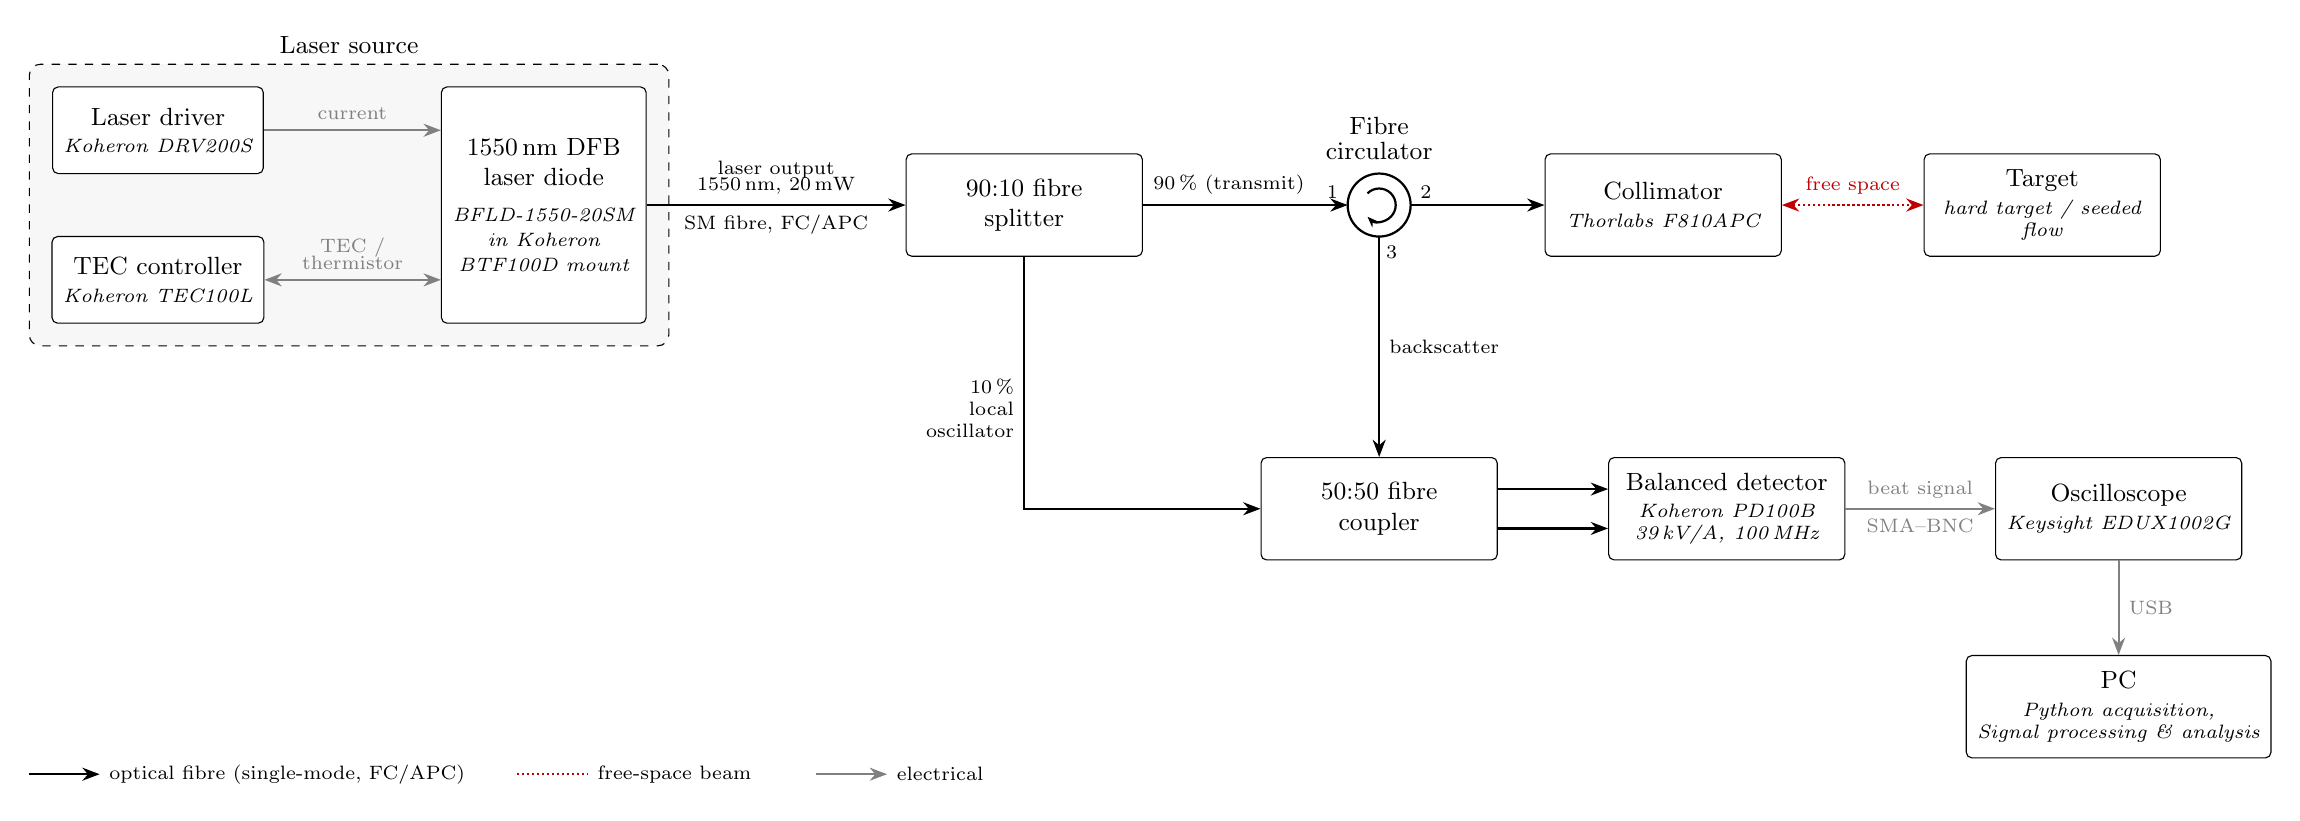
\begin{tikzpicture}[
    font=\small,
    >={Stealth[length=2.2mm]},
    block/.style={draw, rounded corners=2pt, minimum height=1.3cm,
                  minimum width=3.0cm, align=center, inner sep=4pt,
                  fill=white},
    subblock/.style={block, minimum width=2.6cm, minimum height=1.1cm},
    fibre/.style={->, thick},
    freespace/.style={<->, thick, red!75!black, densely dotted},
    elec/.style={->, thick, gray},
    lbl/.style={font=\scriptsize, midway},
  ]
 
  % ======================= laser source (sub-blocks) =======================
  \node[subblock] (drv) at (0,0.95)
    {Laser driver\\[-1pt]{\scriptsize\itshape Koheron DRV200S}};
  \node[subblock] (tec) at (0,-0.95)
    {TEC controller\\[-1pt]{\scriptsize\itshape Koheron TEC100L}};
  \node[subblock, minimum height=3.0cm] (diode) at (4.9,0)
    {1550\,nm DFB\\laser diode\\[2pt]
     {\scriptsize\itshape BFLD-1550-20SM}\\[-2pt]{\scriptsize\itshape in Koheron}\\[-2pt]{\scriptsize\itshape BTF100D mount}};
 
  \draw[elec] (drv.east) -- node[lbl, above] {current} (drv.east -| diode.west);
  \draw[elec, <->] (tec.east) -- node[lbl, above, align=center] {TEC /\\[-2pt]thermistor}
                  (tec.east -| diode.west);
 
  \begin{scope}[on background layer]
    \node[draw, rounded corners=4pt, dashed, inner sep=8pt, fill=gray!6,
          fit=(drv)(tec)(diode), label={[font=\small]above:Laser source}] (src) {};
  \end{scope}
 
  % ======================= transmit row =======================
  \node[block, right=3.0cm of src.east |- diode.east, anchor=west] (split)
    {90:10 fibre\\splitter};
 
  % circulator
  \coordinate (circ) at ($(split.east)+(3.0,0)$);
  \draw[thick, fill=white] (circ) circle (0.40);
  \draw[thick,-{Stealth[length=1.4mm]}] ($(circ)+(135:0.21)$) arc (135:-135:0.21);
  \node[above=0.45cm of circ, align=center] {Fibre\\[-2pt]circulator};
  \coordinate (p1) at ($(circ)+(-0.40,0)$);
  \coordinate (p2) at ($(circ)+(0.40,0)$);
  \coordinate (p3) at ($(circ)+(0,-0.40)$);
  \node[font=\scriptsize, above left=-1pt and 0pt of p1] {1};
  \node[font=\scriptsize, above right=-1pt and 0pt of p2] {2};
  \node[font=\scriptsize, below right=0pt and -1pt of p3] {3};
 
  \node[block, right=2.1cm of circ] (coll)
    {Collimator\\[-1pt]{\scriptsize\itshape Thorlabs F810APC}};
  \node[block, right=1.8cm of coll] (target)
    {Target\\[-1pt]{\scriptsize\itshape hard target / seeded}\\[-3pt]{\scriptsize\itshape flow}};
 
  % ======================= receive row =======================
  \node[block, below=3.2cm of circ] (mix)
    {50:50 fibre\\coupler};
  \node[block, right=1.4cm of mix] (pd)
    {Balanced detector\\[-1pt]{\scriptsize\itshape Koheron PD100B}\\[-3pt]{\scriptsize\itshape 39\,kV/A, 100\,MHz}};
  \node[block, right=1.9cm of pd] (scope)
    {Oscilloscope\\[-1pt]{\scriptsize\itshape Keysight EDUX1002G}};
  \node[block, below=1.2cm of scope] (pc)
    {PC\\[-1pt]{\scriptsize\itshape Python acquisition,}\\[-3pt]{\scriptsize\itshape Signal processing \& analysis}};
 
  % ======================= connections =======================
  % laser output
  \draw[fibre] (diode.east) -- node[lbl, above, align=center]
      {laser output\\[-2pt]1550\,nm, 20\,mW}
      node[lbl, below] {SM fibre, FC/APC} (split.west);
 
  % transmit path
  \draw[fibre] (split) -- node[lbl, above, pos=0.42] {90\,\% (transmit)} (p1);
  \draw[fibre] (p2) -- (coll);
  \draw[freespace] (coll) -- node[lbl, above] {free space} (target);
 
  % local oscillator
  \draw[fibre] (split.south) |- node[lbl, pos=0.3, left, align=right]
      {10\,\%\\local\\oscillator} (mix.west);
 
  % backscatter
  \draw[fibre] (p3) -- node[lbl, right] {backscatter} (mix.north);
 
  % balanced outputs
  \draw[fibre] ([yshift=2.5mm]mix.east) -- ([yshift=2.5mm]pd.west);
  \draw[fibre] ([yshift=-2.5mm]mix.east) -- ([yshift=-2.5mm]pd.west);
 
  % detection chain
  \draw[elec] (pd) -- node[lbl, above] {beat signal} node[lbl, below] {SMA--BNC} (scope);
  \draw[elec] (scope) -- node[lbl, right] {USB} (pc);
 
  % ======================= legend =======================
  \begin{scope}[shift={(src.west |- pc.south)}, yshift=-0.2cm]
    \draw[fibre] (0,0) -- (0.9,0);
    \node[right, font=\scriptsize] at (0.9,0) {optical fibre (single-mode, FC/APC)};
    \draw[freespace, -] (6.2,0) -- (7.1,0);
    \node[right, font=\scriptsize] at (7.1,0) {free-space beam};
    \draw[elec] (10.0,0) -- (10.9,0);
    \node[right, font=\scriptsize] at (10.9,0) {electrical};
  \end{scope}
\end{tikzpicture}}
\caption{Architecture diagram of final system design}
\label{fig:finalDesign}
\end{figure}

\chapter{Noise Analysis}

 \section{Introduction}
 This chapter gives a comprehensive account of the testing which was done on the completed DWL system to account for the various sources of noise. The purpose of the noise analysis is to quantify the noise observed in the system and attribute it to the appropriate sources, while investigating how component, architecture, and operating point choice affects this. This chapter is separate from the functional testing of \autoref{sec:functionalAnalysis}, as the experimental setup differs significantly, and the results from these experiments will indeed be used to inform the expected results of the experiments in \autoref{sec:functionalAnalysis}, and to construct an optimal experimental setup in those cases.

 \section{A: Electronic and Shot Noise}
 
 \subsection{Experimental Goals}
 As discussed in \autoref{sec:lit-noiseSources}, a coherent DWL performs best when it is
 shot-noise limited: the shot noise of the local oscillator (LO) must dominate every other
 noise source at the detector. Experiment A characterises the receiver's noise floor with
 the LO as the only light on the detector, so that the individual noise contributions can be
 separated and measured. It has the following goals:
 
 \begin{itemize}
 	\item \textbf{Measure the electronic noise floor (A1).} With the laser off, measure the
 	noise of the PD100B and acquisition chain alone, and compare it with the input-referred
 	noise specified in the PD100B datasheet. Agreement with the datasheet validates the
 	data collection and post-processing chain used in all later experiments.
 	
 	\item \textbf{Measure shot noise as a function of LO power (A2).} Step the laser drive
 	current to vary the LO power reaching the balanced detector, and confirm that the excess
 	noise above the electronic floor grows linearly with LO power, as expected for shot noise.
 	
 	\item \textbf{Choose the operating point.} From the A2 results, find the LO power at which
 	shot noise overtakes the electronic floor, and choose a laser operating point at which the
 	system is close enough to the shot-noise limit to meet requirement P2
 	(\autoref{tab:requirements}).
 	
 	\item \textbf{Quantify RIN and validate balanced detection (A3).} Repeat the measurement
 	with only one photodiode connected, making the PD100B a single-ended detector. Comparing
 	this with the balanced case measures the laser's relative intensity noise (RIN) and
 	confirms that the balanced detector cancels this common-mode noise as intended. This experiment is only included for completeness, to demonstrate RIN cancellation, and the results are given in Appendix \ref{appendix:RINValidation}.
 \end{itemize} 

 \subsection{Experimental Methodology}
 The experimental setup used is given in \autoref{fig:expASetup}:

 \begin{figure}[H]
 \resizebox{\textwidth}{!}{%
     \centering
 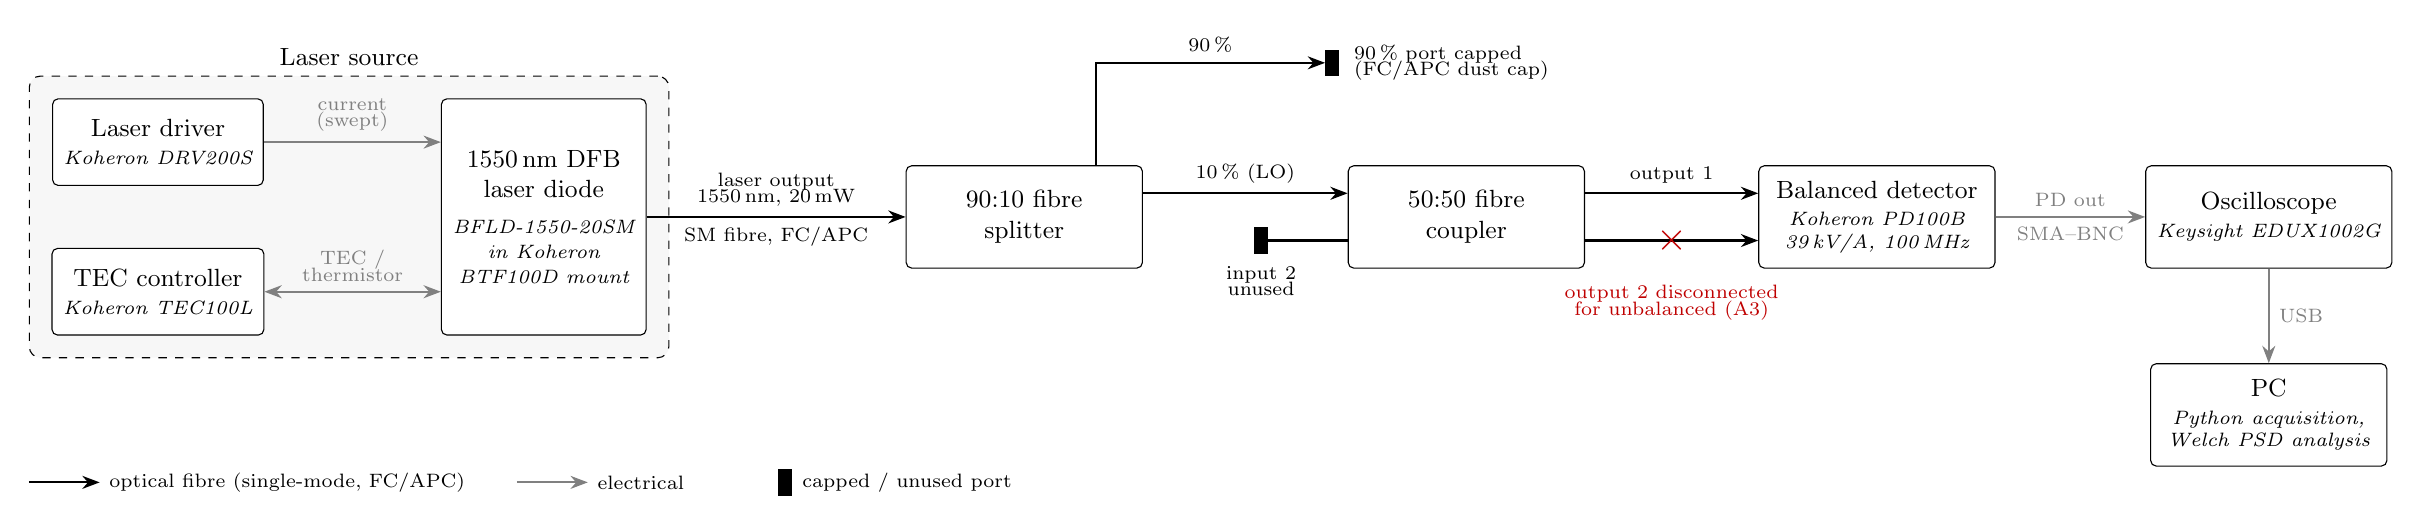
\begin{tikzpicture}[
     font=\small,
     >={Stealth[length=2.2mm]},
     block/.style={draw, rounded corners=2pt, minimum height=1.3cm,
                   minimum width=3.0cm, align=center, inner sep=4pt,
                   fill=white},
     subblock/.style={block, minimum width=2.6cm, minimum height=1.1cm},
     fibre/.style={->, thick},
     elec/.style={->, thick, gray},
     lbl/.style={font=\scriptsize, midway},
     portcap/.style={draw, fill=black, minimum width=1.6mm, minimum height=3.2mm,
                 inner sep=0pt},
   ]
 
   % ======================= laser source (sub-blocks) =======================
   \node[subblock] (drv) at (0,0.95)
     {Laser driver\\[-1pt]{\scriptsize\itshape Koheron DRV200S}};
   \node[subblock] (tec) at (0,-0.95)
     {TEC controller\\[-1pt]{\scriptsize\itshape Koheron TEC100L}};
   \node[subblock, minimum height=3.0cm] (diode) at (4.9,0)
     {1550\,nm DFB\\laser diode\\[2pt]
      {\scriptsize\itshape BFLD-1550-20SM}\\[-2pt]{\scriptsize\itshape in Koheron}\\[-2pt]{\scriptsize\itshape BTF100D mount}};
 
   \draw[elec] (drv.east) -- node[lbl, above, align=center] {current\\[-2pt](swept)}
                  (drv.east -| diode.west);
   \draw[elec, <->] (tec.east) -- node[lbl, above, align=center] {TEC /\\[-2pt]thermistor}
                   (tec.east -| diode.west);
 
   \begin{scope}[on background layer]
     \node[draw, rounded corners=4pt, dashed, inner sep=8pt, fill=gray!6,
           fit=(drv)(tec)(diode), label={[font=\small]above:Laser source}] (src) {};
   \end{scope}
 
   % ======================= optical path =======================
   \node[block, right=3.0cm of src.east |- diode.east, anchor=west] (split)
     {90:10 fibre\\splitter};
 
   % 90 % port capped
   \coordinate (capat) at ($(split.north east)+(2.4,1.3)$);
   \node[portcap] (capnode) at (capat) {};
   \node[right=2pt of capnode, font=\scriptsize, align=left]
     {90\,\% port capped\\[-2pt](FC/APC dust cap)};
 
   \node[block, right=2.6cm of split] (mix)
     {50:50 fibre\\coupler};
 
   % unused coupler input
   \coordinate (unused) at ($([yshift=-3mm]mix.west)+(-1.1,0)$);
   \node[portcap] (capin) at (unused) {};
   \node[below=1pt of capin, font=\scriptsize, align=center] {input 2\\[-2pt]unused};
 
   \node[block, right=2.2cm of mix] (pd)
     {Balanced detector\\[-1pt]{\scriptsize\itshape Koheron PD100B}\\[-3pt]{\scriptsize\itshape 39\,kV/A, 100\,MHz}};
   \node[block, right=1.9cm of pd] (scope)
     {Oscilloscope\\[-1pt]{\scriptsize\itshape Keysight EDUX1002G}};
   \node[block, below=1.2cm of scope] (pc)
     {PC\\[-1pt]{\scriptsize\itshape Python acquisition,}\\[-3pt]{\scriptsize\itshape Welch PSD analysis}};
 
   % ======================= connections =======================
   \draw[fibre] (diode.east) -- node[lbl, above, align=center]
       {laser output\\[-2pt]1550\,nm, 20\,mW}
       node[lbl, below] {SM fibre, FC/APC} (split.west);
 
   \draw[fibre] ([xshift=-6mm]split.north east) |- node[lbl, pos=0.75, above] {90\,\%}
       (capnode.west);
 
   \draw[fibre] ([yshift=3mm]split.east) -- node[lbl, above] {10\,\% (LO)}
       ([yshift=3mm]mix.west);
   \draw[thick] (capin.east) -- ([yshift=-3mm]mix.west);
 
   % coupler outputs -> detector
   \draw[fibre] ([yshift=3mm]mix.east) -- node[lbl, above] {output 1}
       ([yshift=3mm]pd.west);
   \draw[fibre] ([yshift=-3mm]mix.east) -- node[pos=0.5, font=\Large,
       red!75!black] (brk) {$\times$} ([yshift=-3mm]pd.west);
   \node[below=4pt of brk, font=\scriptsize, align=center, red!75!black]
     {output 2 disconnected\\[-2pt]for unbalanced (A3)};
 
   % detection chain
   \draw[elec] (pd) -- node[lbl, above] {PD out} node[lbl, below] {SMA--BNC} (scope);
   \draw[elec] (scope) -- node[lbl, right] {USB} (pc);
 
  
 
   % ======================= legend =======================
   \begin{scope}[shift={(src.west |- pc.south)}, yshift=-0.2cm]
     \draw[fibre] (0,0) -- (0.9,0);
     \node[right, font=\scriptsize] at (0.9,0) {optical fibre (single-mode, FC/APC)};
     \draw[elec] (6.2,0) -- (7.1,0);
     \node[right, font=\scriptsize] at (7.1,0) {electrical};
     \node[portcap] at (9.6,0) {};
     \node[right, font=\scriptsize] at (9.7,0) {capped / unused port};
   \end{scope}
 \end{tikzpicture}}
 \caption{Experimental setup A}
     \label{fig:expASetup}
 \end{figure}

 It can be seen that this differs from the full system setup. The circulator and collimator are unused for this experiment. The 90\% splitter arm is left unconnected and is capped. Only the 10\% splitter arm (LO) is connected to the one arm of the 50:50 coupler. Both outputs of the coupler are connected to the balanced detector, except in the case of experiment A3. Since there is no circulator, collimator or target, the only light reaching the detector is the LO itself. With no second optical field there is no beat term (as in \autoref{eqn:beatSignal}), and the LO contributes only a DC photocurrent, which is removed by the detector's AC coupling. Thus, the signal at the detector will be a pure noise signal, containing only electronic noise and shot noise. Note that phase-induced intensity noise is not present here, as it originates from reflections in the collimator and circulator which are not present in this setup, and RIN is assumed to be cancelled fully by balanced detection.

 The experiment is divided into three phases, with slightly different configurations for each in order to give different measurands, as shown in \autoref{tab:expAParts}:

 \begin{table}[H]
     \centering
     \begin{tabular}{|p{3.5cm}|p{7cm}|p{5cm}|}
     \hline
         \textbf{ID} & \textbf{Configuration} & \textbf{Quantity Measured} \\ \hline
          A1 & Laser output off, detector switched on & Electronic noise only \\ \hline
          A2 & Laser output on (current varied), detector switched on, both detector inputs connected & Electronic noise + shot noise \\ \hline
          A3 (supplementary experiment) & Laser output on (current varied), detector switched on, only one detector input connected & Electronic noise + shot noise + full RIN \\ \hline
     \end{tabular}
     \caption{Experiment A phases and configurations}
     \label{tab:expAParts}
 \end{table}

 For each measurement, the laser is held at a fixed drive current and
 100 records of the detector output are captured sequentially with the oscilloscope and
 transferred to a laptop. Each record contains 25\,000 samples at 125\,MSa/s (200\,$\mu$s).
 A1 requires only a single measurement, while A2 and A3 are repeated over a range of drive
 currents up to the 48\,mA operating point.
 
 The PSD of each record is estimated using Welch's method (Hann window, 2\,500-sample
 segments with 50\,\% overlap, giving a 50\,kHz resolution) rather than a single periodogram,
 since averaging over segments greatly reduces the variance of the estimate, giving a smoother curve. Because the noise
 is stationary (properties don't change across records), the PSDs of the 100 records can then be averaged as well for further smoothing.
 
 To compare the results with a single figure, the PSD can be averaged over the 5--20\,MHz band.
 From \autoref{eq:DopplerShift}, this band corresponds to target speeds of roughly
 4--15.5\,m/s, making it a reasonable band to take an average noise power measurement over, as it is where the Doppler peaks in subsequent tests would appear.

\subsection{Results and Discussion}
\subsubsection{A1: Electronic Noise}
The power spectral density plot in \autoref{fig:A1PSD} was obtained from measurement A1, which gives the electronic noise from the detector only:

\begin{figure}
	\centering
	\includegraphics[width=1\linewidth]{"../Data Acquisition/figures/A1_PSD"}
	\caption{A1: PSD of electronic noise from detector}
	\label{fig:A1PSD}
\end{figure}


The obtained PSD plot is noisy, despite the use of the Welch PSD and averaging, however it is sufficient for the purposes of this investigation. It can be seen that the electronic noise increases with frequency. The average PSD over the 5 - 20MHz band is calculated (using the script) as: $8.06\times 10^{-14}V^2/Hz$. Using the PD100B detector's gain value of 39kV/A, this can be converted into an average input noise current density across 5 - 20MHz, for comparison to the PD100B datasheet:

\begin{equation}
    I_{input} = \frac{8.06\times 10^{-14}V^2/Hz}{(39kV/A)^2}=7.28pA/\sqrt{Hz}
\end{equation}

Input noise current density can be seen as the equivalent of injecting this noise current at the detector input. The calculated average of $7.28pA/\sqrt{Hz}$ across 5 - 20MHz agrees closely with the PD100B's datasheet value of $8pA/\sqrt{Hz}$, measured at 10MHz \cite{Koheron PD100B}. Thus, this level of electronic noise is expected, and the measurement and post processing chain is validated. 

In order to achieve shot-noise limited operation, the average PSD of the shot-noise over this region must thus be $\gg8.06\times 10^{-14}V^2/Hz$.

\subsubsection{A2: Electronic Noise \& Shot Noise}
\autoref{fig:A2PSD} gives the PSD plots of the total noise - made up of shot-noise, electronic noise, and residual RIN - for different laser currents on the same axes:

\begin{figure}
	\centering
	\includegraphics[width=1\linewidth]{"../Data Acquisition/figures/psd_overlay"}
	\caption{PSD of total noise (shot, electronic and relative intensity noise) for different laser source currents}
	\label{fig:A2PSD}
\end{figure}

It can be seen that the total noise increases with increased laser current - this is expected, due to the linear relationship between shot noise and LO power (which is related to laser current which is varied here). In order to compare the PSDs for the various laser currents, the average PSD across the 5 - 20MHz range can again be taken here, for each laser current. \autoref{fig:A2PSDvsCurrent} gives these averages plotted against laser current:

\begin{figure}[H]
    \centering
    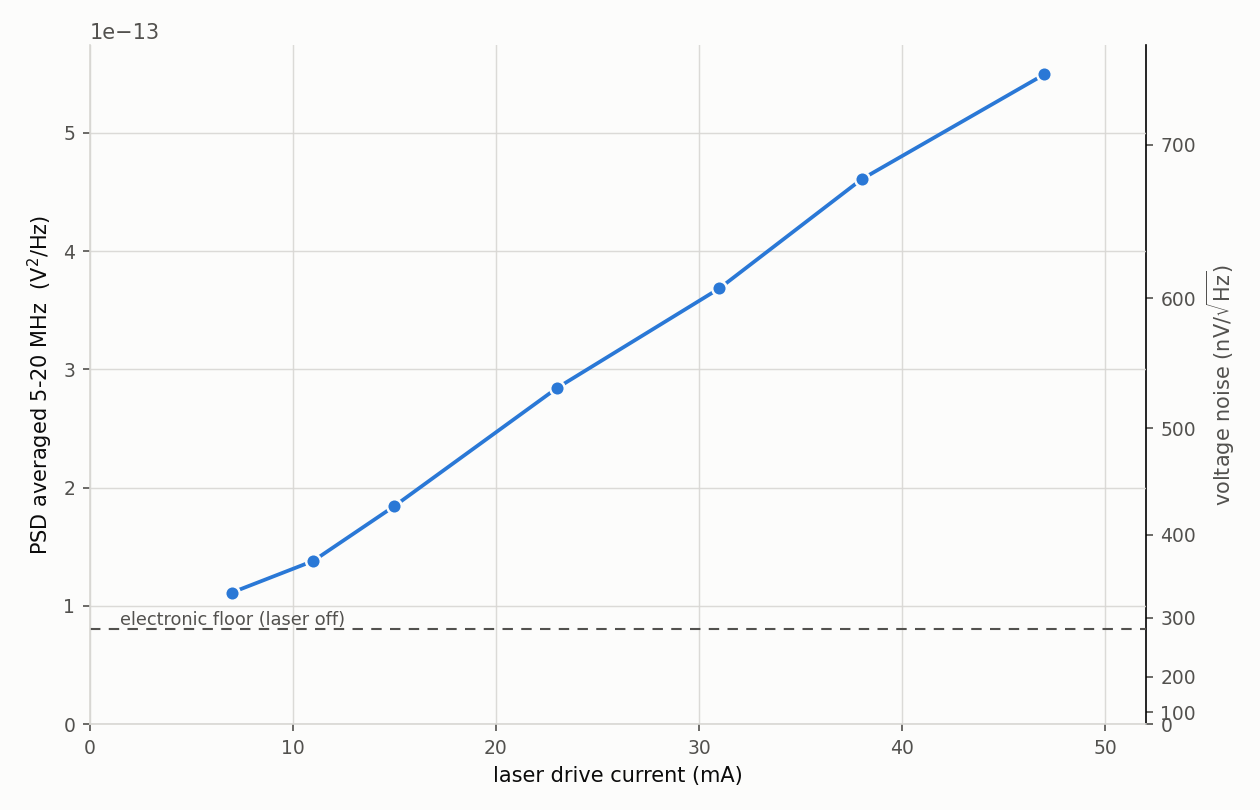
\includegraphics[width=1\linewidth]{psd_vs_current.png}
    \caption{5 - 20MHz Average PSD vs Laser Current with Balanced Detection}
    \label{fig:A2PSDvsCurrent}
\end{figure}

It can clearly be seen in \autoref{fig:A2PSDvsCurrent} and \autoref{fig:A2PSD} that the shot-noise exceeds the electronic noise floor at even the lowest measured laser currents, thus making the system shot-noise limited. As the current is increased, the system approaches the ideal shot-noise limit, as shot noise increasingly swamps out the electronic noise floor. 

Performance requirement P2 in \autoref{tab:requirements} requires that the total detector noise is within 1dB of the shot-noise limit. This requirement can be decomposed as follows:

Noise power adds in linear units, so letting $S$ be shot noise, and $E$ be every other noise source present here (electronic noise and any remaining RIN), the total noise floor, $T$ is given by:
\begin{equation}
    T = S + E = S(1+\frac{E}{S})
\end{equation}

Converting to dB:

\begin{equation}
    10log_{10}(S(1+\frac{E}{S}))=10log_{10}(S) + 10log_{10}(1 + \frac{E}{S})
\end{equation}
In this form, it can clearly be seen that as $S$ increases, the effect of $E$ on the total noise floor is increasingly reduced, as the second term, $10log_{10}(1+\frac{E}{S})$ approaches zero. This second term is the excess noise above the ideal shot-noise limit, which is given by $10log_{10}(S)$. Thus, in order to obtain a total noise floor which is within 1dB of the shot noise limit, we set:

\begin{equation}
    10log_{10}(1+\frac{E}{S})=1dB
\end{equation}
\begin{equation}
    \xrightarrow{}\frac{E}{S}\leq0.26
    \label{eqn:A2Crossover}
\end{equation}

Substituting the obtained electronic noise floor obtained in A1 into \autoref{eqn:A2Crossover}, we obtain:

\begin{equation}
    S \geq 3.1 \times 10^{-13}V^2/Hz
\end{equation}

Noting that \autoref{fig:A2PSD} and \autoref{fig:A2PSDvsCurrent} both give the \textbf{total} detector noise floor (shot \textbf{and} electronic noise), we require the total noise to be above $3.906 \times 10^{-13}V^2/Hz$ to gives a shot noise value of $3.1 \times 10^{-13}V^2/Hz$. This can be seen to be reached at a laser current of approximately 32mA. Above 32mA, the total detector noise floor is within 1dB of the ideal shot-noise limit, and the ideal shot-noise limit is further approached as the current is increased. 

From this, it can be seen that an operating current of 48mA for the laser allows P2 in \autoref{tab:requirements} to be met with the highest margin, and this will thus be used as the laser current for the remainder of this project. While a higher laser current still may be used, to even further approach the ideal shot-noise limit, this risks saturating the detector. The detector has a maximum incident power rating of 1.5mW on each photodiode \cite{detector  datasheet}. From the laser datasheet \cite{laser datasheet}, a current of 48mA gives approximately 17mW at the laser output, which will result in approximately 0.85mW at each detector from the LO alone. This allows the detector to thus remain comfortably far away from its saturation point, even if returned signal is high and results in a higher incident power at the photodiode after mixing with the LO. 

\subsubsection{A3: Relative Intensity Noise}
Experiment A3 serves only for completeness, to illustrate the effectiveness of balanced detection in removing relative intensity noise at the detector output. It was found that indeed 0.6125dB of RIN was cancelled by using the balanced detection setup. See Appendix \ref{appendix:RINValidation} for the full results and discussion of this supplementary experiment.  

\section{B: Phase-induced Intensity Noise}
\subsection{Experimental Goals}
As discussed in \autoref{sec:lit-noiseSources}, and elaborated in Appendix \ref{appendix:PIIN}, Phase-induced Intensity Noise (PIIN) can be a significant contributor to the total noise of the system, rising far above shot-noise - particularly when the linewidth of the laser source is not narrow, and when there is significant path-length mismatch between the LO and the transmit signal.

 The goal of Experiment B is to measure and quantify the magnitude and shape of the total noise of the system, including PIIN, in a controlled setting. There is effectively no target in this experiment, thus making all PIIN in the measurement attributable to reflections from the circulator and collimator, and independent of target. 
 
 
 \subsection{Experimental Methodology}
 For this experiment, the system is set up in full, as given by the final design in \autoref{fig:finalDesign}. The collimator is then pointed at a stationary matte-black painted surface, angled 45 degrees away from the collimator, and at a distance of 10cm from the collimator. Any reflections from the target surface will not be Doppler shifted, because it is stationary - thus, if these reflections are sent back into the collimator, they will appear at the output as additional PIIN (see Appendix \ref{appendix:PIIN}). This setup thus intends to absorb and reflect a large amount of the emitted light \textbf{away} from the system, so that the measured PIIN can be attributed to only the internal reflections in the system from the collimator and circulator, which is independent of target. 
 
 The laser is then driven with a current of 48mA (the chosen operating point for LO power), and the same oscilloscope acquisition chain and post-processing chain (Welch PSD) as in experiment A is used to obtain the PIIN power. As discussed in \cite{jiang_performance_2019}, PIIN can vary drastically depending on temperature, or small disturbances in the system's fiber optics, thus this measurement is repeated 16 times over the course of an hour to account for such variations. The average noise power as well as the spread from these measurements can then be computed. 
 
 \subsection{Results and Discussion}
 \autoref{fig:psdpiin} below gives the averaged PSD of the obtained noise measurements, with the electronic noise floor and the total noise floor (excluding PIIN) from Experiment A2 given as reference. 
 
\begin{figure}[H]
	\centering
	\includegraphics[width=1\linewidth]{"../Data Acquisition/figures/psd_piin"}
	\caption{Experiment B: Total noise in the system, including PIIN}
	\label{fig:psdpiin}
\end{figure}

 It can be seen that the total noise is now significantly above that measured in A2, owing to the excess noise introduced by PIIN. It can also be seen that as expected, PIIN varied significantly between measurements. In the 5 - 20MHz band, the total excess noise was measured to be from 12.2 to 14.2dB above the A2 noise floor, for a given frequency. It can also be seen that this excess noise is not constant, and starts rolling off steeply from approximately 10MHz. The shape of the PIIN corresponds to the $L_c \gg \Delta L$ regime described in Appendix \ref{appendix:PIIN}, as it is a flat floor and does not contain a Lorentzian peak at baseband.
 
 From these results it is thus clear that in this system, PIIN dominates other noise sources by a large amount, especially at lower frequencies. It is thus the largest single noise contributor in the total SNR of the system when trying to measure a Doppler peak, and the system is therefore no longer shot-noise limited (the ideal case).  
 
 \subsection{Reducing PIIN}
 The experiments in \autoref{sec:functionalTesting} were performed using the system as is, with the PIIN-limited behaviour observed and described above. It was found that while the system could adequately detect the velocity of a hard-target, it did not have enough sensitivity to detect the velocity of a seeded air-flow, owing to the high noise floor from PIIN. It was thus decided that an attempt would be made to reduce PIIN, from the theory discussed in \autoref{sec:lit-noiseSources} and elaborated in Appendix \ref{appendix:PIIN}. Obtaining a narrower linewidth laser source is out of budget for this project, thus the only remaining option was to attempt to better match the fiber optic path length between the LO and the received signal. This allows the LO and the received signal to be more coherent in phase at the detector. This is because the travel-time for both will be closer matched, meaning that the phase of the laser will not have been able to "wander" by as much between the two signals.
 
 FC/APC fiber patch cords of varying lengths were obtained and inserted in between the 10\% splitter arm and the one arm of the 50:50 mixer, to effectively increase the LO path length, in an attempt to closer match the longer path length followed by the received signal (which traverses the collimator and free-space twice, in excess of the LO path). The PIIN of the system was measured for each length of patch-cable using the same methodology previously described, with 10 averages for each patch cable length. The results are given in \autoref{fig:psdpiinlengths}:
 
\begin{figure}
	\centering
	\includegraphics[width=1\linewidth]{"../Data Acquisition/figures/psd_piin_lengths"}
	\caption{Total noise in the system for different inserted patch-cable lengths}
	\label{fig:psdpiinlengths}
\end{figure}

It can be seen that 
\chapter{Functional Testing}
\label{sec:functionalTesting}
This chapter details the testing which was done on the system's primary function: velocity measurement. Two distinct test setups are used, which are described in this section - results were then collected for these test setups and are presented and discussed with respect to the goals of the system and the overarching project. 

\section{C: Hard-target Speed Measurement}
\subsection{Experimental Goals}
The overarching goal of the system is to measure wind-speed via the Doppler shift, however, owing to the very weak signal return in air and complexities in setting up appropriate tests, this is a challenging test to perform. For this reason it was decided that before wind-speed measurement testing is performed, hard-target speed measurement would first be tested. This uses the same working principle as wind-speed measurement, but with a target which provides a far higher signal return. Thus, this experiment serves to first validate the working principle of the system to measure velocity via the optical Doppler shift, before wind-speed measurement testing is performed. This allows for any significant setup or procedure problems in the system to be identified in an environment which is easier to control, and which is more reliable for measurement (owing to the larger return signal, and thus higher SNR). 

\subsection{Experimental Methodology}
In order to generate a constant and precise hard-target velocity to be measured, a NEMA-17 stepper motor is used with a disc attached to the motor shaft. Stepper motors are capable of rotating at very constant and accurate RPMs. If the motor axis is tilted at an angle with respect to the laser beam, there will be a component of the disc's angular velocity in the direction of the laser beam. If the beam is carefully aligned with a known point on the disc's radius, the instantaneous velocity of that point in the direction of the beam, $v_{los}$, can thus be calculated. A design was created and 3D printed, which aligns the collimator lens with a spot on the spinning disc's radius. \autoref{fig:CRig} shows the setup used:
\begin{figure}[H]
	\centering
	\includegraphics[width=1\linewidth]{../../../../../Downloads/fig_rig_side3d}
	\caption{Test setup used for hard-target speed measurement}
	\label{fig:CRig}
\end{figure}
As shown in the figure, an angle of 45 degrees is used between the collimator and the motor axis, and the beam is aimed approximately $d = 15mm$ from the centre of the disc. The line of sight velocity of the beam is thus: $v_{los}=sin(45)2\pi N \times d$, where $N$ is the RPM of the motor, and $d$ is the radius from the centre of the disc to the beam spot. While care was taken in the design to precisely align the collimator with the intended point at $d=15mm$, any error in this alignment will translate directly into a measured velocity which is different from the calculated velocity. Furthermore, the beam spot has a finite size which has a diameter of approximately 7mm (from the F810-APC datasheet \cite{f810 apc datasheet}) - thus the measurement will also have contributions from other points on the disc radius which move at a different angular velocity to the intended target point. These contributions are likely to appear as a broadening of the Doppler peak. 

It must also be noted that the PLA plastic used reflects very little light at 1550nm, and thus standard white paper was attached to the spinning disc to increase the reflectivity. 

The rest of the system is set up as in \autoref{fig:finalDesign}, with all components fully connected. The laser is driven at a constant 48mA.

The motor RPM is varied across measurements in order to test the system's ability to resolve various different speeds. The same data acquisition and processing chain as for experiments A and B are used here, with 100 oscilloscope records being obtained for a given motor RPM, their Welch PSDs computed, and averaged to obtain a result. 

\subsection{Results and Discussion}

\begin{figure}[H]
	\centering
	\includegraphics[width=1\linewidth]{"../Data Acquisition/figures/psd_rpm_overlay"}
	\caption{C: PSD of hard-target speed measurements, at different motor RPMs}
	\label{fig:CPSD}
\end{figure}

\begin{figure}
	\centering
	\includegraphics[width=1\linewidth]{"../Data Acquisition/figures/peak_vs_rpm"}
	\caption{C: Doppler peak frequency (from centroid) vs target motor RPM}
	\label{fig:CentroidVSRPM}
\end{figure}

\begin{table}[H]
	\centering
	\small
	\setlength{\tabcolsep}{4pt}
	\caption{Doppler peak and local noise floor for each target speed (capture~1 of each speed,
		Welch PSD with $\Delta f = \SI{10}{kHz}$). $f_D$ is the power-weighted centroid of
		the excess PSD over the stationary-target reference, and
		$v_{\mathrm{LOS}} = f_D / (\SI{1.29}{MHz.s/m})$. The PSD at $f_D$ is that of the bin
		nearest the centroid; the noise statistics are taken in a band outside
		$3\times$FWHM around the centroid, out to \SI{2}{MHz} either side. All PSD values are
		in the same units, so the PSD at $f_D$ can be compared directly with the detection
		threshold (mean $+\,5\sigma$), which it exceeds at every speed. The excess power is the PSD above the local
		noise, integrated across the peak.}
	\label{tab:doppler_vs_rpm}
	\smallskip

	\begin{tabular}{
			|S[table-format=4.0]   % RPM
			|S[table-format=1.3]   % f_D (centroid)
			|S[table-format=1.3]   % v_LOS
			|S[table-format=1.2]   % mean noise
			|S[table-format=1.2]   % mean + 5 sigma
			|S[table-format=2.1]   % PSD at f_D
			|S[table-format=2.1]   % PSD/mean
			|S[table-format=1.2]|  % integrated excess power
		}
		\hline
		\multicolumn{1}{|c|}{\textbf{Speed}} & \multicolumn{1}{c|}{\boldmath$f_D$} & \multicolumn{1}{c|}{\boldmath$v_{\mathrm{LOS}}$}
		& \multicolumn{3}{c|}{\textbf{PSD} (\num{e-11}\,\si{V^2/Hz})} & \multicolumn{1}{c|}{\textbf{PSD/mean}} & \multicolumn{1}{c|}{\textbf{Excess power}} \\ \cline{4-6}
		\multicolumn{1}{|c|}{(RPM)} & \multicolumn{1}{c|}{(\si{MHz})} & \multicolumn{1}{c|}{(\si{m/s})}
		& \multicolumn{1}{c|}{Mean noise} & \multicolumn{1}{c|}{Mean $+\,5\sigma$}
		& \multicolumn{1}{c|}{\textbf{At \boldmath$f_D$}} & \multicolumn{1}{c|}{(\si{dB})} & \multicolumn{1}{c|}{(\num{e-5}\,\si{V^2})} \\ \hline
		50 & 0.079 & 0.061 & {7.01\textsuperscript{\dag}} & 9.35 & 50.7 &  8.6 & 4.09 \\ \hline
		100 & 0.164 & 0.127 & {2.56\textsuperscript{\dag}} & 3.95 & 75.7 & 14.7 & 4.00 \\ \hline
		200 & 0.330 & 0.256 & {1.43\textsuperscript{\dag}} & 2.24 & 78.6 & 17.4 & 4.35 \\ \hline
		600 & 0.996 & 0.772 & 4.92 & 7.86 & 26.1 &  7.2 & 3.76 \\ \hline
		800 & 1.331 & 1.032 & 5.61 & 8.99 & 25.2 &  6.5 & 3.91 \\ \hline
		1200 & 1.985 & 1.539 & 4.07 & 6.38 & 14.5 &  5.5 & 3.63 \\ \hline
		2000 & 3.314 & 2.569 & 2.92 & 4.06 & 10.4 &  5.5 & 3.93 \\ \hline
	\end{tabular}
	
	\vspace{2pt}
	\raggedright\footnotesize
	\textsuperscript{\dag}\,Peak too close to DC for a noise band below it; the floor is taken
	from the high-frequency side only and is likely a slight underestimate.
\end{table}

\section{C: Wind-speed Measurement}
\subsection{Experimental Goals}
Now that the noise analysis of the system is complete, and the speed-measurement principle has been shown to be functional for a hard-target, the system can finally be tested for seeded air wind-speed measurement. The primary subject of investigation for this section is the sensitivity of the system with respect to its noise and the different levels of seeding in the air, as well as its accuracy at different tested speeds. As discussed previously, the range of the system can not be tested in a wind-tunnel environment, and thus this is out of scope for this project. 
\subsection{Experimental Setup}
% Wind-tunnel test set-up (side view). Coordinates are in mm, scaled 1 mm -> 0.25 mm.
% Needs: \usepackage{tikz} \usetikzlibrary{arrows.meta,patterns,decorations.pathmorphing,calc}
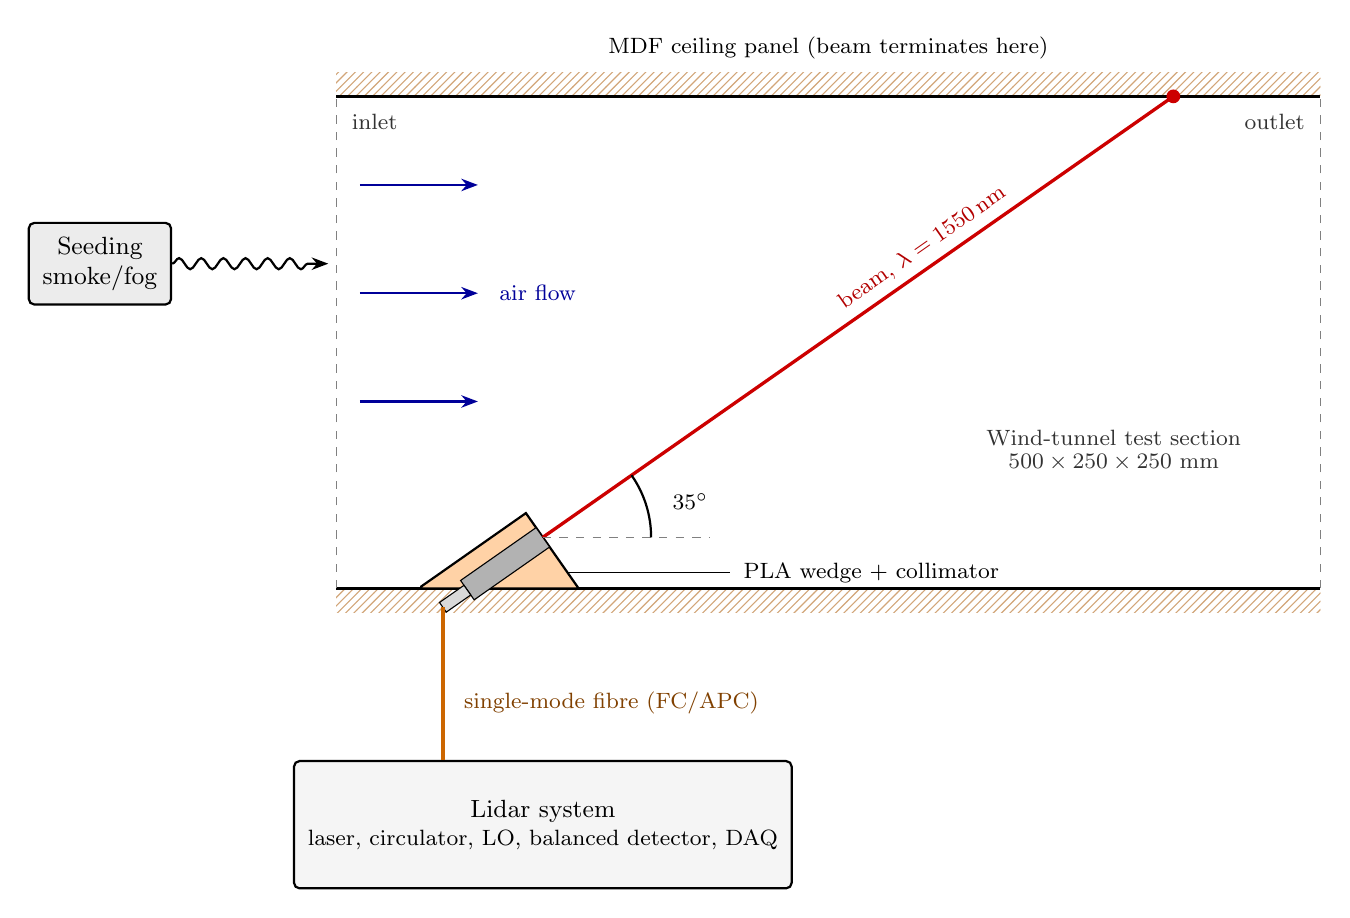
\begin{tikzpicture}[x=0.25mm, y=0.25mm, font=\small,
	blk/.style={draw, thick, rounded corners=2pt, align=center, fill=gray!8, inner sep=5pt},
	flow/.style={-{Stealth[length=6pt]}, thick, blue!60!black},
	lbl/.style={font=\footnotesize, align=center}]
	
	% ---------------- wind-tunnel test section ----------------
	\fill[pattern=north east lines, pattern color=brown!70] (0,250) rectangle (500,262);
	\fill[pattern=north east lines, pattern color=brown!70] (0,-12) rectangle (500,0);
	\draw[very thick] (0,250) -- (500,250);
	\draw[very thick] (0,0) -- (500,0);
	\draw[dashed, gray] (0,0) -- (0,250);
	\draw[dashed, gray] (500,0) -- (500,250);
	\node[lbl, anchor=south] at (250,264) {MDF ceiling panel (beam terminates here)};
	\node[lbl, anchor=north west, gray!40!black] at (3,246) {inlet};
	\node[lbl, anchor=north east, gray!40!black] at (497,246) {outlet};
	\node[lbl, gray!40!black] at (395,70) {Wind-tunnel test section\\[-1pt]$500 \times 250 \times 250$~mm};
	
	% air-flow arrows
	\foreach \y in {95,150,205} \draw[flow] (12,\y) -- (72,\y);
	\node[lbl, blue!60!black, anchor=west] at (78,150) {air flow};
	
	% ---------------- seeding ----------------
	\node[blk, fill=gray!15] (seed) at (-120,165) {Seeding\\smoke/fog};
	\draw[-{Stealth[length=6pt]}, thick, decorate,
	decoration={snake, amplitude=2pt, segment length=8pt, post length=6pt}]
	(seed.east) -- (-4,165);
	
	% ---------------- wedge and collimator ----------------
	% printed PLA wedge (side profile), lens centre at (105,26)
	\filldraw[fill=orange!35, draw=black, thick]
	(43.2,0) -- (43.2,1.0) -- (96.4,38.3) -- (123.2,0) -- cycle;
	% collimator body along the beam axis (35 deg), lens face at (105,26)
	\begin{scope}[shift={(105,26)}, rotate=35]
		\filldraw[fill=gray!60, draw=black] (-46.8,-6) rectangle (0,6);
		\filldraw[fill=gray!30, draw=black] (-62,-3) rectangle (-46.8,3);   % FC/APC connector
	\end{scope}
	\draw[thin] (200,8) -- (118,8);
	\node[lbl, anchor=west] at (202,8) {PLA wedge + collimator};
	
	% ---------------- beam ----------------
	\draw[red!80!black, very thick] (105,26) -- (425.3,250);
	\fill[red!80!black] (425.3,250) circle (3.5);
	\path (105,26) -- (425.3,250) node[pos=0.62, sloped, above, lbl, red!70!black] {beam, $\lambda = \SI{1550}{nm}$};
	
	% angle to the flow
	\draw[dashed, gray] (105,26) -- (190,26);
	\draw[thick] (160,26) arc[start angle=0, end angle=35, radius=55];
	\node[lbl] at (180,44) {$35^\circ$};
	
	% ---------------- fibre and lidar system ----------------
	\node[blk, minimum width=150, minimum height=46] (sys) at (105,-120)
	{Lidar system\\[-1pt]{\footnotesize laser, circulator, LO, balanced detector, DAQ}};
	\coordinate (rear) at ($(105,26)+(215:62)$);
	\draw[orange!80!black, very thick] (rear) -- (rear |- sys.north);
	\node[lbl, orange!50!black, anchor=west] at (60,-58) {single-mode fibre (FC/APC)};
\end{tikzpicture}


\chapter{Conclusions and Recommendations}
\label{sec:conclusionsAndRecommendations}
This report has demonstrated a working benchtop-scale Doppler wind LiDAR,
built from readily available components. The conclusions from each
experiment are given first, followed by a table summarising the findings of the report with respect to the performance requirements, and thereafter recommendations for improving the
system are given; each conclusion refers to the recommendations that address it.

\section{Conclusions}

 Firstly, it can be seen in the noise analysis that while the system was able to achieve shot-noise limited operation with respect to the electronic noise of the detector (thus meeting requirement P1), this was not maintained once PIIN was introduced. The final system was PIIN limited; after matching fiber path lengths, internal PIIN was measured at an average of approximately 5.7dB above the shot-noise level, with significant variation and instability in this noise being seen across measurements. Prior to matching fiber path lengths, PIIN was measured at 22.1dB above shot noise. This illustrates the importance of path-length matching in reducing PIIN to acceptable levels, but also highlights that despite matching the path-lengths, the system is still 5.7dB above the optimal sensitivity which can be reached, which is the shot-noise limit. See recommendation R1 for suggested improvements on this. 

Thereafter, the functional analysis yielded several important results. It was firstly verified that the system is capable of hard target velocimetry, with Doppler peaks detected at 16.9 - 25.9dB above the noise floor, at less than 1000 PSD averages (thus meeting P4). While the wind-tunnel could not be used for testing the minimum resolvable LOS speed, a hard-target speed of 0.056m/s was measured in Experiment C, thus meeting the low-end requirement of P5.

 After validating the system's working principle on a hard-target, testing of wind-speed measurement was conducted. It was found that the system produced measurable Doppler peaks above the detection threshold at all tested wind-speeds between 3 - 21m/s, for dense fog seeded air, at less than 10 000 PSD averages, thus meeting P6 and the high-end requirement of P5. The time taken to acquire this amount of averages to obtain a result is shown to be in line with acquisition times in commercial systems when the oscilloscope's bottleneck is ignored, however recommendation R2 discusses the implementation of a data acquisition chain which does not have this same bottleneck. The system was also tested using lighter mist-seeded air. For this test case, it was found that the returned signal power was far lower, and that the system only reached the detection threshold after approximately 21 600 independent PSD averages. This illustrates the benefits of increased averages in lowering the detection threshold by lowering noise variance. However, crucially, it was found that the system built as is would require an impractical $10^5$ times more averages for peak detection in unseeded air with yet still lower signal return power. This is attributed to the lack of an optical power amplifier in the system, and the high PIIN. Recommendation R1 and R3 discuss improvement paths relating to this. 
 
 It was also found that the system's Doppler peak measurements, when converted to velocity, overshot the expected velocity values relative to the wind-tunnel setpoint by approximately 10\%, thus failing requirement P7 on velocity error being within 5\%. Further experimentation however showed that this error could partially be attributed to the test-rig geometry, and could be reduced via a single-point calibration. After the calibration, the error was approximately 1.1\%, and thus within the bounds to meet P7. Recommendation R4 discusses this matter further.
 
 Ultimately, the contents of this report effectively demonstrate the working principles of a Doppler wind LiDAR system and quantifies its detection sensitivity and velocity accuracy with respect to the noise in the system and the components used.
 
 A summary of the results with respect to the requirements laid out in \autoref{sec:design-sysReqs} is given in \autoref{tab:req-verification}:
 
 \begin{table}[H]
 	\centering
 	\small
 	\setlength{\tabcolsep}{4pt}
 	\renewcommand{\arraystretch}{1.2}
 	\begin{tabular}{@{} l
 			>{\raggedright\arraybackslash}p{0.27\linewidth}
 			>{\raggedright\arraybackslash}p{0.38\linewidth}
 			>{\raggedright\arraybackslash}p{0.12\linewidth}
 			l @{}}
 		\toprule
 		\textbf{ID} & \textbf{Requirement} & \textbf{Result} & \textbf{Verdict} & \textbf{Section} \\
 		\midrule
 		P1 & Detector noise within 1 dB of the shot-noise limit
 		& 0.72 dB above the shot-noise limit at 48 mA
 		& Met & 4.2 \\
 		P2 & PIIN level and spectral shape measured; low enough for P6
 		& Flat floor, 22.1 dB above shot-noise limit, reduced to 4.3 dB by path-length matching; enabled P6
 		& Met & 4.3 \\
 		P3 & Total system noise quantified and attributed
 		& 5.7 dB above shot-noise limit; dominated by PIIN (\autoref{tab:noise-budget})
 		& Met & 4.3, 4.4 \\
 		P4 & Hard-target peak $\geq 5\sigma$ above mean at $N \leq 1000$
 		& 16.9--25.9 dB above the noise mean at all six speeds, $N \approx 245$
 		& Met & 5.1 \\
 		P5 & LOS speed range $\leq 0.1$ to $\geq 15$ m/s
 		& 0.056 m/s resolved (C); 17.2 m/s resolved (D)
 		& Met & 5.1, 5.2 \\
 		P6 & Seeded-air peak $\geq 5\sigma$ above mean at $N \leq 10\,000$
 		& Dense fog: detected at all nine speeds, $N \approx 7200$. Light mist (5 m/s): required $N \approx 21\,600$
 		& Met (fog); not met (mist) & 5.2 \\
 		P7 & Velocity within 5\,\% of ground truth
 		& $+10.6$\,\% (C), $+10.7$\,\% (D) as built; 1.1\,\% RMS after one-point calibration
 		& Met after calibration & 5.1, 5.2 \\
 		\bottomrule
 	\end{tabular}
 	\caption{Verification of the performance requirements of \autoref{tab:requirements}.}
 	\label{tab:req-verification}
 \end{table}

\section{Recommendations}
From the concluded results discussed above, a number of recommendations can be made for future work on this system. These recommendations form an essential part of the project's work, as they are derived from quantified limitations in the current system. 

\begin{enumerate}[label=\textbf{R\arabic*}]
	\item \textbf{Narrow linewidth laser source: } It is recommended that a narrower linewidth laser source in the order of 50 - 100kHz is obtained. This serves to reduce PIIN, which currently raises the noise floor to approximately 5.7dB above the shot-noise floor, and which is highly unstable, so that the total noise of the system is reduced to approximately 0.6dB above the optimal shot-noise level. This will increase the detection sensitivity of the system, and increase its ability to resolve turbulence via a narrower Doppler peak. \\
	
	\item  \textbf{High sample-rate ADC and FPGA processing chain:} The current setup uses an oscilloscope and laptop as the processing chain. While the oscilloscope can sample at a high enough rate, it has a data transfer bottleneck which results in measurements being taken across a time period of 30 - 60 seconds, with only approximately 0.2\% of data in this period actually being sampled and used. It is thus recommended that instead an ADC and FPGA processing chain can be developed, which samples continuously and performs the necessary FFT calculations at a high rate. This can increase the data usage for a given time period up to 100\% \cite{hill_remote_nodate}, thus reducing the acquisition time to be in the order of 100ms, and giving the system a sample rate of up to 10Hz, which is in line with commercial systems and real-world wind conditions.\\
	
	\item \textbf{Optical power amplifier: } The system as is does not emit a very high power laser beam (approximately 15mW), and the returned backscatter power is thus very low, limiting the system's ability to measure Doppler peaks in clear, unseeded air. It is recommended that an optical power amplifier (ideally an EDFA) be added so as to increase the emitted power, and thus increase the system's sensitivity and detection ability. \\
	
	\item \textbf{Test environment flow-profiling: } It is recommended that a wind-tunnel test environment's flow is comprehensively profiled, and that a test-rig which minimally interferes with this flow is designed, so that the accuracy of the system can be better tested and quantified and does not rely on calibration for accurate measurements in a controlled environment. \\
	
	\item  \textbf{Focusing optics: } It is recommended that focusing optics are added after the collimator lens. This would allow the system to achieve ranging of the measured wind-speeds, rather than averaging the flow equally over the entire beam. \\
	
	\item \textbf{Acousto-optic modulator: } It is recommended that an acousto-optic modulator be added to the system. This converts the system to a heterodyne, rather than homodyne detection system, and would thus allow for the resolution of the direction of the velocity, rather than just the magnitude. This is essential for real-world applications where the flow direction is not known, as it was in this report's test environment.

\end{enumerate}


 


%\chapter{Recommendations}

Make sensible recommendations for further work.

\bibliographystyle{plain} 
\bibliography{Bibliography-25Aug}
\appendix
% ============================================================
% Master file for the appendices.
% In the main document, replace the old
%     \appendix
%     \include{Appendix A}
%     \include{Addenda}
% (or whatever the template uses) with:
%     \appendix
%     \input{appendices/appendices}
%
% Order follows the first reference to each appendix in the body of the
% report. Appendix A is fixed by the template (GA summary).
% ============================================================
\chapter{Graduate Attributes}
\label{appendix:GA}

The table below summarises how the graduate attributes (GAs) associated with this course have been met, and where in the report the evidence can be found.

\setlength{\LTcapwidth}{\linewidth}
\begin{longtable}{|>{\centering\arraybackslash}p{0.05\linewidth}
		|>{\raggedright\arraybackslash}p{0.17\linewidth}
		|p{0.66\linewidth}||}
	\caption{Graduate attributes and where they are addressed in this report}
	\label{tab:GAs}\\
	\hline
	\textbf{GA} & \textbf{Requirement} & \textbf{Justification and section in the report} \\ [0.5ex]
	\hline\hline
	\endfirsthead
	
	\multicolumn{3}{l}{\small\itshape \tablename~\thetable{} (continued)}\\
	\hline
	\textbf{GA} & \textbf{Requirement} & \textbf{Justification and section in the report} \\ [0.5ex]
	\hline\hline
	\endhead
	
	\hline
	\multicolumn{3}{r}{\small\itshape Continued on next page}\\
	\endfoot
	
	\hline
	\endlastfoot
	
	1 & Problem-solving & My project concerns the field of LiDAR for wind-speed measurement. Specifically, my project deals
	with the problem of designing a prototype benchtop-scale version of a Doppler wind LiDAR system. I
	consulted various sources of literature in order to first understand what the key use-cases and goals of
	Doppler wind LiDAR systems are (mostly with respect to wind-turbines, and the use of such systems to
	control the turbines optimally). Thereafter, with the end-use in mind, I reviewed sources which discuss
	common types/classes of such systems (\autoref{sec:litReview}), and identified a system type which would be suitable for this
	project, given the time-frame and budget -- this type being coherent detection Doppler LiDAR (\autoref{sec:design-sysArch}).
	After identifying this suitable class of system, I reviewed the various design considerations of such a
	system in the available literature (\autoref{sec:litReview}). This included mathematical and physical descriptions of how the
	system operates, with respect to signal theory, optics, electronics, and relevant physics phenomena
	(including Rayleigh and Mie scattering, coherent detection methodology, balanced detection, and
	laser source physics). From this, I synthesised a list of parts which would be suitable for use in the project, and used the relevant mathematics to validate these choices in terms of the final
	requirements (\autoref{sec:design-ComponentChoices}, \autoref{sec:design-sysReqs}).
	\\
	\hline
	4 & Investigations, experiments and data analysis & I conducted a thorough investigation into the various types of Doppler wind LiDAR systems which are
	used in industry and scientific research. After doing so, I conducted more specific research into
	coherent detection Doppler LiDAR systems, and the physics, signal processing and optics which
	underpin these systems (\autoref{sec:litReview}, \autoref{sec:design-ComponentChoices}). From this, I was able to recommend to my supervisor a course of action for
	the class of system to be designed, and substantiate this choice through the research done.
	I formulated various experiments to conduct on the system once it
	was built, which validate the signal theory, mathematics and electronics principles
	concerned, and validate the system's workings (\autoref{sec:noiseAnalysis}, \autoref{sec:functionalTesting}). The primary consideration in these experiments is a thorough noise analysis (\autoref{sec:noiseAnalysis}), which
	serves to quantify the sensitivity of the system. Furthermore, the effects of various design decisions on the
	performance (e.g.\ source laser linewidth and power, or the use of balanced detection over single-ended detection) are analysed in these experiments, and optimal requirements for such systems
	are thus experimentally shown and discussed, and suitable recommendations for upgrades are made. \\
	\hline
	5 & Use of engineering tools & Engineering mathematics was used in the system's design in order to determine the optimal components to use (e.g.\ the fibre-optic splitter ratio in \autoref{sec:design-ComponentChoices}). Reasoning based on the reviewed literature was applied to predict performance outcomes and to determine how the system should be tested (e.g.\ the prediction that the system will require seeded air for wind-speed measurement due to the lack of optical power amplification, \autoref{sec:design-ComponentChoices}). Once the system was built, an oscilloscope was used in conjunction with Python scripts to acquire data from the system (setup described in \autoref{sec:design-DataAcquisition}, used in \autoref{sec:noiseAnalysis} and \autoref{sec:functionalTesting}). The data was also post-processed using Python scripts so as to gain useful information from it, and to generate plots and tables which show the obtained data in a readable manner. \\
	\hline
	6 & Professional and technical communication (long report) & I have attended scheduled meetings (and scheduled further follow-up meetings) with my supervisor in
	order to discuss the route which the project should take, as well as budget and technological
	considerations. I have also consulted with Maysam Soltanian to obtain suitable sources for components
	which are required for the project.
	
	This written project report serves to communicate the technical details of the system's development and testing to an engineering audience. The abstract and conclusion of this report serve to communicate basic ideas (e.g.\ the need for system upgrades in order to perform wind-speed measurements in clean air) to a non-engineering or management audience. \\
	\hline
	8 & Individual work & I have maintained goals and suggested timeframes for my work on the project. While meetings
	with my supervisor and Maysam helped guide the sourcing and budget constraints for the project
	components, all of the specific components were selected by me, and suitable sourcing suggestions
	were made to Maysam. While the supervisor provided the overarching topic of Doppler wind LiDAR, I
	used my own research into the area to select an appropriate subclass of LiDAR system to build for the
	project, synthesising the constraints of the project and the desired requirements. All experimental work was synthesised individually. Appendix \ref{appendix:AIUse} shows a knowledge of professional ethics and norms in its declaration of how and where artificial intelligence was used in this project. \\
	\hline
	9 & Independent learning ability & I have independently learnt concepts in photonics (laser source characteristics), atmospheric sciences
	(Rayleigh and Mie scattering) and signal theory (coherent detection and balanced detection), in order
	to understand and synthesise the design of a Doppler wind LiDAR system.
	
	The initial problem was ill-defined and the decision to take the route of designing a benchtop-scale
	Doppler wind LiDAR system was not immediately obvious. It was only after learning more about the
	field and evaluating areas of research in it that this decision was made, after reaching out to my
	supervisor to consult on this. Throughout the project I have had to manage the scope of the project to
	suit my abilities and constraints, given that the field of research contains many complexities which are
	beyond an undergraduate skill-level and time-frame. This therefore shows my ability to synthesise
	meaningful objectives, knowledge and outcomes from an ill-posed problem. \\ [1ex]
\end{longtable}
   % A  GA summary (template-mandated)
\chapter{Linewidth, PIIN and Doppler Peak Broadening}
\label{appendix:PIIN}
% Referenced from: Sec 2.5 (noise sources), Sec 3.4.1 (Linewidth),
% Table 3.1 (monostatic row -- change its \autoref{sec:lit-linewidth} to
% \autoref{appendix:PIIN}), Sec 4.3.1, Sec 4.3.3 (fix the "Appendix ??" there
% to \autoref{appendix:PIIN}), Sec 4.3.4.
In order to understand the linewidth property of a laser source, it is important to first have an understanding of the concept of phase noise in a laser:

    An ideal laser emits an electromagnetic wave $E(t) = E_0cos(2\pi f_0t + \phi)$ with $\phi$ a constant. A real laser emits $E(t)=E_0cos(2\pi f_0t + \phi(t))$ where $\phi(t)$ drifts unpredictably. This drift is called phase noise. Thus, when considering the frequency spectrum of the emitted laser beam over a long time period, it takes a Lorentzian shape centred around the nominal frequency of the laser (whereas an ideal laser would present simply as a delta spike at the nominal frequency). The laser linewidth, $\Delta f$, is then defined as the -3dB bandwidth of this Lorentzian spectrum, as illustrated in \autoref{fig:lorentzian} below:

    \begin{figure}[H]
    \centering
    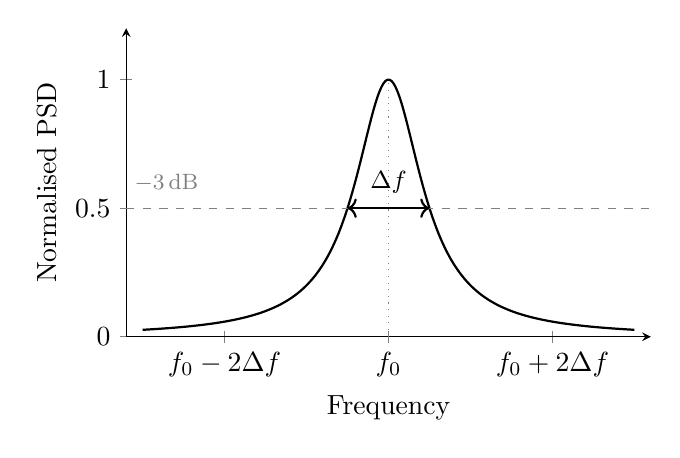
\begin{tikzpicture}
    \begin{axis}[
        width=0.68\textwidth, height=5.5cm,
        xlabel={Frequency},
        ylabel={Normalised PSD},
        domain=-3:3, samples=400,
        xmin=-3.2, xmax=3.2, ymin=0, ymax=1.2,
        axis lines=left,
        xtick={-2,0,2},
        xticklabels={$f_0-2\Delta f$, $f_0$, $f_0+2\Delta f$},
        clip=false,
    ]
    \addplot[thick, black] {1/(1+(2*x)^2)};

    % half-maximum level
    \addplot[dashed, gray] coordinates {(-3.2,0.5) (3.2,0.5)};
    \node[left, gray, font=\footnotesize] at (axis cs:-2.2,0.6) {$-3$\,dB};

    % centre line
    \draw[dotted, gray] (axis cs:0,0) -- (axis cs:0,1);

    % FWHM arrow
    \draw[<->, thick] (axis cs:-0.5,0.5) -- (axis cs:0.5,0.5);
    \node[above, font=\small] at (axis cs:0,0.52) {$\Delta f$};
    \end{axis}
    \end{tikzpicture}
    \caption{Lorentzian frequency spectrum of a laser diode.}
    \label{fig:lorentzian}
    \end{figure}

    Asssociated with the linewidth is a quantity termed coherence length. The coherence length of the emitted beam, $L_c$, is given by \cite{bennett_doppler_2003}:

    \begin{equation}
        L_c = \frac{c}{2\pi\Delta f}
        \label{eqn:coherenceLength}
    \end{equation}

    Where $\Delta f$ is the linewidth of the source laser, and $c$ is the speed of light. The coherence length is of relevance when considering linewidth effects.

    The non-ideal linewidth property of a laser source gives rise to two primary effects in a DWL system's measurements - namely phase-induced intensity noise (PIIN), and the broadened Doppler peak:

    As noted by Cariou et al. \cite{cariou2006laser}, Jiang et al. \cite{jiang_performance_2019}, and Harris et al. \cite{harris_role_1998}, reflections of the outgoing beam - caused by optics and the fibre optic transmit path - travel back in the system and are interfered with the reference beam (LO) before detection (in the same way as the actual backscattered signal of interest is). Because the reflection and LO derive
    from the same source, the mixing product is a strong, unwanted tone at baseband (homodyne)
    or at the intermediate frequency (heterodyne), carrying the phase noise
    accumulated over the path-length mismatch $\Delta L$ between the reflection and the LO. Harris et
    al. \cite{harris_role_1998} show that the form of this residual noise is set by how large
    $\Delta L$ is relative to the coherence length ($L_c$) of the laser source.

    For $\Delta L \gg L_c$ the two
    phases are highly uncorrelated because the difference in path (and therefore time) taken has allowed the phase of the two to "wander" significantly - and thus the tone broadens into a Lorentzian of width
    $2\Delta f$. This case is illustrated in \autoref{fig:commonmode} below, where it can be seen that this unwanted Lorentzian peak can serve to swamp out the desired Doppler peak to be measured - this is especially impactful for low wind-speeds, where the Doppler peak will be closer to the unwanted common-mode Lorentzian peak, and will be hidden more by it.

    \begin{figure}[H]
    \centering
    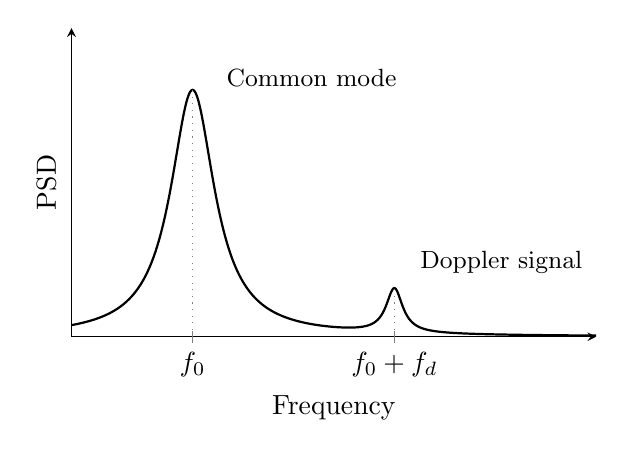
\begin{tikzpicture}
    \begin{axis}[
        width=0.68\textwidth, height=5.5cm,
        xlabel={Frequency},
        ylabel={PSD},
        domain=-1.5:5, samples=500,
        xmin=-1.5, xmax=5, ymin=0, ymax=1.25,
        axis lines=left,
        xtick={0,2.5},
        xticklabels={$f_0$, $f_0+f_d$},
        ytick=\empty,
        clip=false,
    ]
    % common mode + Doppler signal
    \addplot[thick, black] {1/(1+(3*x)^2) + 0.18/(1+(8*(x-2.5))^2)};

    % centre lines
    \draw[dotted, gray] (axis cs:0,0) -- (axis cs:0,1);
    \draw[dotted, gray] (axis cs:2.5,0) -- (axis cs:2.5,0.2);

    % peak labels
    \node[right, font=\small] at (axis cs:0.3,1.05) {Common mode};
    \node[right, font=\small] at (axis cs:2.7,0.3) {Doppler signal};
    \end{axis}
    \end{tikzpicture}
    \caption{Spectrum of a monostatic CW coherent lidar, showing the Doppler
    signal superimposed on the skirt of the common-mode peak (adapted from \cite{cariou2006laser}).}
    \label{fig:commonmode}
    \end{figure}

    For $\Delta L \ll L_c$, the case where the mismatch between LO and reflection paths is smaller, the reflected signal and the LO will be more correlated in phase.
    Thus, the residual instead appears as a flat excess noise floor across the
    frequency band, of level proportional to $\Delta f\,\Delta L^{2}$
    \cite{harris_role_1998}. This excess noise is termed excess LO noise,
    interferometric noise or phase-induced intensity noise (PIIN), depending on author
    \cite{harris_role_1998,abari_all-fiber_2014,jiang_performance_2019}. For the remainder of this paper, this excess noise will be termed PIIN. PIIN has
    been measured at 5 - 30dB above shot noise in a diode-laser
    lidar \cite{harris_role_1998} and well above shot noise in a fibre-laser
    system \cite{jiang_performance_2019}. Thus, PIIN is a significant noise source which can cause the system to operate far from the ideal shot-noise limit discussed in \autoref{sec:lit-noiseSources}. It is thus clear that to reduce PIIN, a laser with as small a linewidth as possible should be selected, and the path length mismatch, $\Delta L$ between LO and reflection paths should be minimised.

    Another consideration arising due to non-ideal laser linewidth is the broadening of the measurable Doppler peak. This is particularly notable for longer ranges.

    If the coherence length from \autoref{eqn:coherenceLength} is long relative to the emitted signal's path length, the broadening of the Doppler peak due to the laser's linewidth may be neglected, and it will instead be other factors (such as turbulence in the air, and speckle) which dominate and cause a broader measurable peak \cite{bennett_doppler_2003}. This is because the total round-trip time of the beam is shorter, thus ensuring that the phase of the beam has not had "time" to shift significantly in between transmission, and later reception and mixing with the local oscillator. Thus, the received backscatter signal and the LO phase will be more coherent and will result in a sharper peak after mixing.

    Conversely, if the coherence length is short relative to the signal path length (i.e. for targets at greater ranges), the Doppler peak will be spread over $2\times\Delta f$, meaning that the measurement resolution and the ability to resolve turbulence in the air will be reduced \cite{bennett_doppler_2003}.

    From the two effects described above, it can clearly be seen that a narrow linewidth laser source is highly beneficial for DWL systems, in order to achieve the best-case shot-noise limited operation, and to achieve a narrow, measurable Doppler peak.
        % B  first ref: Sec 2.5
\chapter{Balanced Detection}
\label{appendix:RIN}
% Referenced from: Sec 2.6, Table 3.1 (balanced-detection row), Sec 5.1.3 and
% Sec 5.2.3 (via \autoref{eq:beat_power}).
As discussed  in \autoref{sec:lit-noiseSources}, the best-case performance of a DWL system is for it to operate in a shot-noise limited regime - thus, all other sources of noise should be reduced to below the shot-noise level. In coherent detection LiDAR architectures, the use of a balanced detector setup has become common for this purpose, as it assists in reducing a laser source's relative-intensity noise (RIN) below the shot-noise level, in a manner which single-ended detection does not.

A single-ended detection system simply uses a 2:1 (2 inputs, one output) fiber optic coupler to mix the LO reference signal with the backscatter signal, and uses a single photodetector to convert this light signal into a measurable current. It can be seen that this detection method retains the DC terms $P_{LO}$, $P_{RS}$. Any RIN from the laser source is present in the output, as these intensity fluctuations are contained in these two power terms. Thus, the measurable Doppler peak will be smaller with respect to the noise floor.

Contrastingly, balanced detection setup makes use of a 2:2 fibre optic coupler which also optically mixes the LO reference signal with the received backscatter signal (as discussed in \autoref{sec:lit-coherentDetection}). However, the 2:2 coupler has two outputs, thus giving two output signals which can be termed $E_1$ and $E_2$ \cite{kikuchi_fundamentals_2016}:

\begin{equation}
	E_1 = \frac{1}{\sqrt2}(E_{RS} + E_{LO}), \space
	E_2 = \frac{1}{\sqrt{2}}(E_{RS} - E_{LO})
\end{equation}
Where $E_{RS}$ and $E_{LO}$ are the complex electromagnetic fields of the returned backscatter signal and the local oscillator respectively.

Thereafter, the two signals enter the balanced detector, which consists of two matched photodiodes and a transimpedance amplifier to convert their currents into a measurable voltage. The photodiodes respond with currents $I_1$ and $I_2$ respectively, proportional to the intensity of the electromagnetic field incident on it ($|E_{1}|^2$ and $|E_2|^2$ respectively), as was also discussed in \autoref{sec:lit-coherentDetection}. Due to the internal setup of the transimpedance amplifier and the photodiodes in the balanced detector, the output current is then given by \cite{kikuchi_fundamentals_2016}:

\begin{equation}
	I_{det} \propto I_1 - I_2 \propto |E_1|^2 - |E_2|^2 \newline
	\propto 2\sqrt{P_{LO}P_{RS}} cos(2\pi\Delta f t)
\end{equation}

Comparing this to \autoref{eqn:beatSignal}, it can be seen that the DC terms $P_{LO}$ and $P_{RS}$ are no longer present due to them being common-mode in both $I_1$ and $I_2$ and thus being canceled by the subtraction. This therefore lowers the noise floor, as the RIN contained in these terms is also eliminated.

Writing in the photodiode responsivity $R$ and the transimpedance gain $G$ of
the balanced detector, the output voltage of the detector is
\begin{equation}
	V(t) = G\,(I_1 - I_2) = 2GR\sqrt{P_{LO}P_{RS}}\,\cos(2\pi\Delta f\,t),
	\label{eq:beat_voltage}
\end{equation}
where $P_{LO}$ and $P_{RS}$ are the total LO and received powers entering the
coupler.

It must also be noted that since the mean of $\cos^2$ is $\tfrac{1}{2}$, the mean-square voltage of the beat signal is
\begin{equation}
	\langle V^2 \rangle = 2G^2R^2P_{LO}P_{RS}.
	\label{eq:beat_power}
\end{equation}
Thus, by Parseval's theorem, $\langle V^2 \rangle$ equals the PSD integrated across
the Doppler peak, so a measured excess power can allow one to estimate the received signal power:
$P_{RS} = \langle V^2 \rangle / (2G^2R^2P_{LO})$.


\autoref{fig:balanceddetector} depicts the balanced detection process graphically:
\begin{figure}[H]
	\centering
	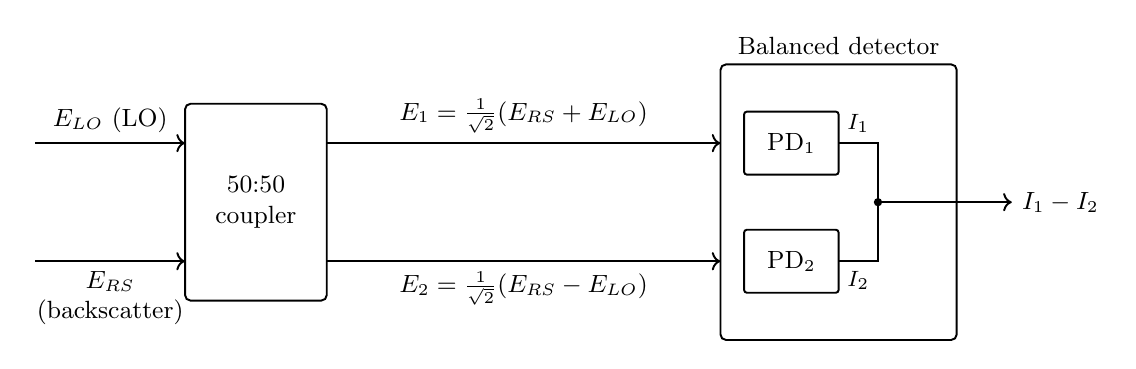
\begin{tikzpicture}[font=\small, line width=0.7pt]

		% ---- inputs ----
		\draw[->] (0.3,2.25) -- (2.2,2.25);
		\node[above] at (1.25,2.25) {$E_{LO}$ (LO)};
		\draw[->] (0.3,0.75) -- (2.2,0.75);
		\node[below, align=center] at (1.25,0.75) {$E_{RS}$\\(backscatter)};

		% ---- coupler ----
		\draw[rounded corners=2pt] (2.2,0.25) rectangle (4.0,2.75);
		\node[align=center] at (3.1,1.5) {50:50\\coupler};

		% ---- coupler outputs ----
		\draw[->] (4.0,2.25) -- (9.0,2.25);
		\node[above] at (6.5,2.25) {$E_1 = \tfrac{1}{\sqrt{2}}(E_{RS} + E_{LO})$};
		\draw[->] (4.0,0.75) -- (9.0,0.75);
		\node[below] at (6.5,0.75) {$E_2 = \tfrac{1}{\sqrt{2}}(E_{RS} - E_{LO})$};

		% ---- balanced detector ----
		\draw[rounded corners=2pt] (9.0,-0.25) rectangle (12.0,3.25);
		\node[above] at (10.5,3.25) {Balanced detector};
		\draw[rounded corners=1pt] (9.3,1.85) rectangle (10.5,2.65);
		\node at (9.9,2.25) {PD$_1$};
		\draw[rounded corners=1pt] (9.3,0.35) rectangle (10.5,1.15);
		\node at (9.9,0.75) {PD$_2$};

		% ---- difference ----
		\draw (10.5,2.25) -- (11.0,2.25) -- (11.0,0.75) -- (10.5,0.75);
		\node[above, font=\footnotesize] at (10.75,2.25) {$I_1$};
		\node[below, font=\footnotesize] at (10.75,0.75) {$I_2$};
		\fill (11.0,1.5) circle (1.5pt);
		\draw (11.0,1.5) -- (12.0,1.5);

		% ---- output ----
		\draw[->] (12.0,1.5) -- (12.7,1.5);
		\node[right] at (12.7,1.5) {$I_1 - I_2$};
	\end{tikzpicture}
	\caption{Balanced detection. The 50:50 coupler delivers the sum and difference
		of the backscatter and LO fields to two matched photodiodes; the output is the
		difference of their photocurrents, in which the common-mode terms cancel and
		only the beat term $2\sqrt{P_{LO} P_{RS}}\cos(2\pi\Delta f t)$ remains.}
	\label{fig:balanceddetector}
\end{figure}

It can thus be seen that balanced detection provides the advantage of cancelling RIN. This allows for the final detected signal to theoretically be able to achieve the desired shot-noise limited operation (if other sources of noise are also eliminated).
      % C  first ref: Sec 2.6
\chapter{Laser Source Classes: Noise and Practical Notes}
\label{appendix:laserSourceNotes}
% Referenced from: Table 3.3 caption (\autoref{tab:laser-sources-notes}).
% Needs the array and booktabs packages (already loaded for Table 3.1).
\begin{table}[H]
\centering\small
\renewcommand{\arraystretch}{1.2}
\begin{tabular}{@{}>{\raggedright\arraybackslash}p{0.22\textwidth}>{\raggedright\arraybackslash}p{0.76\textwidth}@{}}
\toprule
\textbf{Source type} & \textbf{Noise and practical notes} \\
\midrule
Fabry--P\'erot laser diode &
Oscillates on several longitudinal modes simultaneously, so the output is not single-frequency and cannot be mixed coherently with a local oscillator; unsuitable for coherent detection \cite{harris_role_1998}. \\
\addlinespace
DFB laser diode &
Single-frequency, but with a linewidth of the order of MHz, which gives rise to significant PIIN in a CW system unless the LO and transmit path lengths are closely matched (\autoref{sec:testingPIIN}). Relaxation-oscillation peak at $\sim$\SI{1}{\giga\hertz}, far above the Doppler band, so RIN is flat and low in the frequency band of interest \cite{cariou2006laser}. Supplied as a bare butterfly module; needs an external current driver and temperature controller. Selected for this project. \\
\addlinespace
Planar external-cavity semiconductor &
kHz-range linewidth, so PIIN and Doppler-peak broadening are greatly reduced compared to a DFB diode. Supplied with an integrated driver, and marketed specifically for wind lidar. \\
\addlinespace
Er-doped DFB fibre laser &
The common source of choice for CW anemometry owing to its very narrow linewidth \cite{cariou2006laser,hill_remote_nodate,abdelazim_development_2015}. Relaxation-oscillation peak near \SI{1}{\mega\hertz}, however, so RIN is higher in the frequency band of interest than for a DFB diode \cite{cariou2006laser}. \\
\bottomrule
\end{tabular}
\caption{Noise and practical notes for the laser source classes compared in \autoref{tab:design-laser-sources}.}
\label{tab:laser-sources-notes}
\end{table}
    % D  first ref: Table 3.3 caption
\chapter{Component Datasheets}
\label{appendix:datasheets}
% Referenced from: Table 3.4 caption (\autoref{appendix:laser}) and
% Table 3.7 caption (\autoref{appendix:pd100b}). The driver, TEC and
% collimator sections are not referenced yet; either add "Full specifications
% are given in \autoref{appendix:driver}" etc. to their captions, or delete the
% sections you don't want.
%
% For each component either \includegraphics the datasheet page(s) or use
%   \includepdf[pages=-]{...}   (needs \usepackage{pdfpages})
% The datasheet files are in the project:
%   Laser Diode Datasheet.jpeg
%   koheron_drv200s-laser-diode-driver.pdf
%   koheron_tec100l-tec-controller.pdf
%   koheron_btf100-butterfly-laser-diode-mount.pdf
%   koheron_pd100b-photodetection.pdf
%   (collimator: Thorlabs F810APC-1550 spec sheet, not yet in the project)

\section{DFB Laser Diode (BFLD-1550-20SM-FA2)}
\label{appendix:laser}
% TODO: insert laser diode datasheet (Laser Diode Datasheet.jpeg)

\section{Laser Driver (Koheron DRV200S-A-200) and Butterfly Mount (BTF100D)}
\label{appendix:driver}
% TODO: insert driver datasheet (koheron_drv200s-laser-diode-driver.pdf) and
% mount datasheet (koheron_btf100-butterfly-laser-diode-mount.pdf)

\section{Temperature Controller (Koheron TEC100L-50)}
\label{appendix:tec}
% TODO: insert TEC controller datasheet (koheron_tec100l-tec-controller.pdf)

\section{Balanced Photodetector (Koheron PD100B-AC)}
\label{appendix:pd100b}
% TODO: insert detector datasheet (koheron_pd100b-photodetection.pdf)

\section{Fibre Collimator (Thorlabs F810APC-1550)}
\label{appendix:collimator}
% TODO: insert collimator spec sheet
            % E  first ref: Table 3.4 caption
\chapter{Supplementary Results: Experiment A}
\label{appendix:expA}

\section{A2: 5--20\,MHz Average PSD per Laser Current}
\label{appendix:A2Table}
% Referenced from: Sec 4.2.3 ("table of results in Appendix ??") -- change that
% to \autoref{appendix:A2Table}.
% TODO: add a table of the data plotted in Figure 4.3, one row per drive
% current (7, 11, 15, 23, 31, 38, 48 mA plus laser-off), with columns for the
% 5-20 MHz averaged PSD (V^2/Hz) and the equivalent voltage noise (nV/sqrt(Hz)).

\section{A3: Supplementary Experiment on RIN Cancellation}
\label{appendix:RINValidation}
% Referenced from: Sec 4.2.1 and Sec 4.2.3 (A3 paragraph).
\autoref{fig:A3Plot} gives the 5 - 20MHz averaged PSD of the detected noise, when only a single photodetector input of the PD100B is used - effectively turning it into a singe-ended detector. The electronic noise floor will remain the same, but the total noise PSD averages will now also contain RIN in addition to shot-noise and electronic noise. Before analysis of this plot can commence, it is important to note that in the case of balanced detection, the shot-noise of each detector is uncorrelated, and will therefore add together at the output. Thus, in the single-ended case, the shot-noise at the output for a given laser current is expected to be half that of the balanced detection case. Any excess noise above this half-power shot-noise level is thus contributed from the electronic noise, and the uncancelled RIN.

\begin{figure}[H]
	\centering
	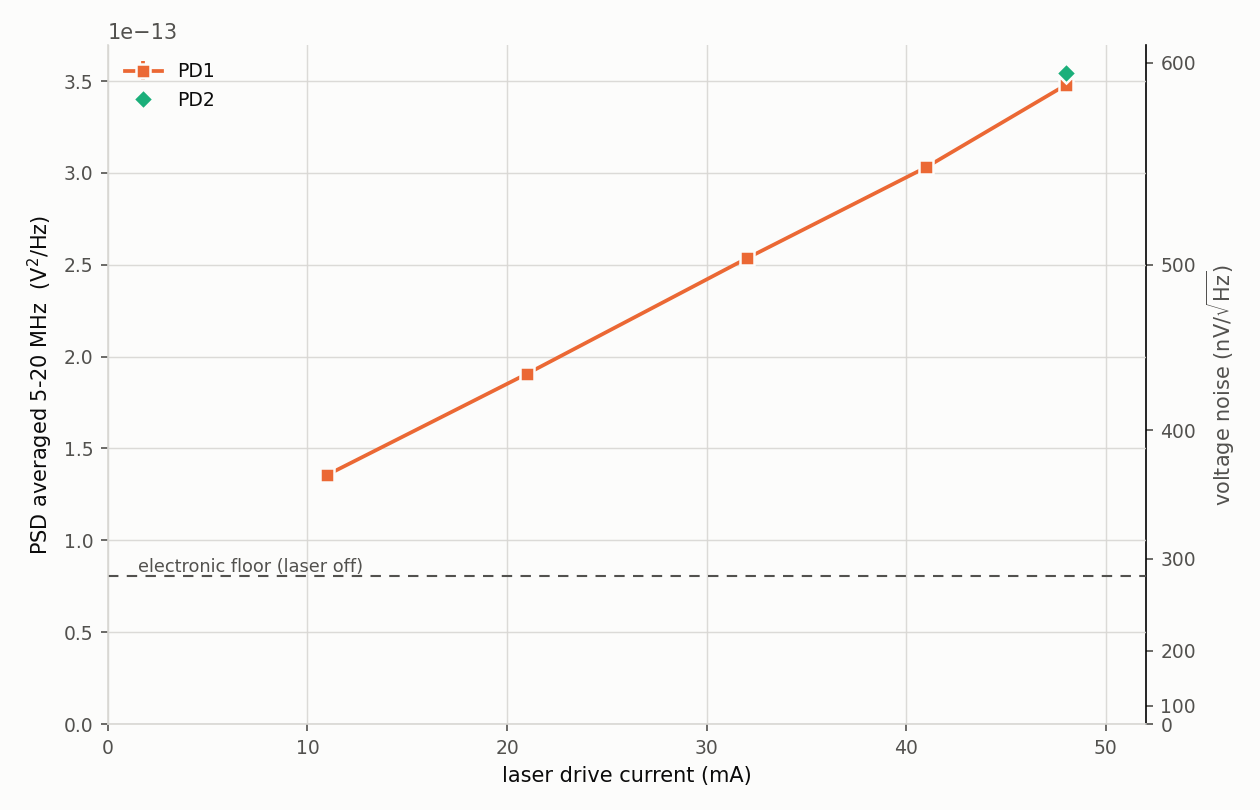
\includegraphics[width=1\linewidth]{psd_vs_current_single.png}
	\caption{A3: 5 - 20MHz Average PSD vs Laser Current with Single-Ended Detection}
	\label{fig:A3Plot}
\end{figure}

It can be seen in \autoref{fig:A3Plot} that indeed, the total noise is lower than in \autoref{fig:A2PSDvsCurrent}, as expected. Observing the total noise at the operating point of 48mA however, it can be seen that a value of approximately $3.5 \times 10^{-13}V^2/Hz$ is obtained, which gives $2.694\times 10^{-13}V^2/Hz$ once electronic noise has been subtracted. In the balanced detection case at the same laser current, a value of $5.49\times10^{-13}V^2/Hz$ was obtained - subtracting electronic noise and halving this gives $2.342\times 10^{-13}V^2/Hz$. This clearly indicates that the noise power in the single-ended case is higher than simply half of the shot-noise in the balanced detection case, thus proving that indeed there is excess RIN present. This excess RIN noise can be calculated:
\begin{equation}
	RIN_{excess}= (2.694 - 2.342)\times 10^{-13} = 0.352\times 10 ^{-13}V^2/Hz
\end{equation}

Converting to dB:

\begin{equation}
	10log_{10}(1+\frac{RIN_{excess}}{S})=10log_{10}(1+\frac{0.352\times 10 ^{-13}}{2.324\times 10^{-13}})= 0.6125dB
\end{equation}

Thus, RIN contributes an additional 0.6125dB of noise above the ideal shot-noise limit at the 48mA operating point. Balanced detection allows this excess noise to be removed, as illustrated in the results of A2 - allowing for a better SNR.
      % F  first ref: Sec 4.2.1
\chapter{Supplementary Results: Experiment D}
\label{appendix:FullWTResults}
% Referenced from: Sec 5.2.3 ("See Appendix ... for the raw PSDs of each case
% plotted on their own axes, and full tables of raw results"), and the captions
% of Tables 5.2 and 5.3 ("Full raw statistics are given in ...").

\section{Raw PSDs per Wind-tunnel Setpoint}
\label{appendix:WTPSDs}
\begin{figure}[H]
	\centering
	\includegraphics[width=0.7\linewidth]{"../Data Acquisition/figures/psd_windtunnel_cases"}
	\caption{Grid of PSD plots for each wind-tunnel setpoint}
	\label{fig:psdwindtunnelcases}
\end{figure}

\section{Raw Noise and Peak Statistics}
\label{appendix:WTRawStats}
% >>> generated: WTRawStats -- written by "Data Acquisition/make_appendixG_tables.py"; edits between these markers are overwritten
\autoref{tab:WTRawStats-fog} and \autoref{tab:WTRawStats-mist} give the un-normalised counterparts of \autoref{tab:D_snr} and \autoref{tab:D_mist_avg}: the same Doppler peaks and noise bands, but with the statistics taken on the raw PSD rather than on the PSD divided by its running-median floor. Because the raw floor slopes across the noise band, its standard deviation here includes that slope as well as the random fluctuation, which makes the raw mean $+\,5\sigma$ threshold the more conservative of the two.

\begin{table}[H]
	\centering
	\small
	\begin{tabular}{@{}S[table-format=2.1] S[table-format=2.3] S[table-format=1.2] S[table-format=1.3] S[table-format=1.2] S[table-format=1.2] S[table-format=1.2] S[table-format=2.2]@{}}
		\toprule
		{Setpoint} & {$f_D$} & \multicolumn{4}{c}{PSD ($10^{-12}$\,V$^2$/Hz)} & {Peak/mean} & {Excess} \\
		\cmidrule(lr){3-6}
		{(m/s)} & {(MHz)} & {floor mean} & {floor $\sigma$} & {mean $+\,5\sigma$} & {at $f_D$} & {(dB)} & {($10^{-7}$\,V$^2$)} \\
		\midrule
		3.1 & 3.637 & 3.01 & 0.078 & 3.41 & 4.73 & 1.96 & 10.25 \\
		5.0 & 5.868 & 3.45 & 0.075 & 3.82 & 4.79 & 1.43 & 8.87 \\
		6.0 & 6.892 & 2.44 & 0.031 & 2.59 & 3.78 & 1.90 & 7.55 \\
		7.0 & 7.997 & 2.30 & 0.040 & 2.50 & 3.49 & 1.82 & 7.04 \\
		8.0 & 9.280 & 4.30 & 0.082 & 4.71 & 5.36 & 0.95 & 5.99 \\
		9.0 & 10.611 & 2.74 & 0.042 & 2.95 & 3.60 & 1.19 & 6.08 \\
		10.0 & 11.664 & 4.20 & 0.054 & 4.46 & 5.18 & 0.92 & 6.00 \\
		11.8 & 13.837 & 3.94 & 0.053 & 4.20 & 4.51 & 0.59 & 5.27 \\
		21.0 & 24.674 & 3.69 & 0.052 & 3.95 & 4.22 & 0.59 & 4.01 \\
		\bottomrule
	\end{tabular}
	\caption{D: raw (un-normalised) noise and Doppler-peak statistics for dense fog-seeded air}
	\label{tab:WTRawStats-fog}
\end{table}

\begin{table}[H]
	\centering
	\small
	\setlength{\tabcolsep}{4.5pt}
	\begin{tabular}{@{}S[table-format=1.1] S[table-format=1.0] S[table-format=2.3] S[table-format=1.2] S[table-format=1.3] S[table-format=1.2] S[table-format=1.2] S[table-format=1.2] S[table-format=2.2]@{}}
		\toprule
		{Setpoint} & {Captures} & {$f_D$} & \multicolumn{4}{c}{PSD ($10^{-12}$\,V$^2$/Hz)} & {Peak/mean} & {Excess} \\
		\cmidrule(lr){4-7}
		{(m/s)} & {averaged} & {(MHz)} & {floor mean} & {floor $\sigma$} & {mean $+\,5\sigma$} & {at $f_D$} & {(dB)} & {($10^{-7}$\,V$^2$)} \\
		\midrule
		5.0 & 1 & 5.730 & 4.48 & 0.090 & 4.93 & {4.80\textsuperscript{\dag}} & 0.30 & 4.38 \\
		5.0 & 2 & 5.716 & 3.83 & 0.087 & 4.27 & {4.08\textsuperscript{\dag}} & 0.28 & 4.45 \\
		5.0 & 3 & 5.726 & 4.00 & 0.081 & 4.41 & {4.29\textsuperscript{\dag}} & 0.30 & 3.75 \\
		\bottomrule
	\end{tabular}

	\vspace{2pt}
	{\raggedright\footnotesize \textsuperscript{\dag}\,PSD at $f_D$ below the raw mean $+\,5\sigma$ threshold. The detection verdicts in \autoref{tab:D_mist_avg} use the floor-normalised PSD instead, on which the \SI{5}{m/s} peak clears its threshold with three captures.\par}
	\caption{D: raw (un-normalised) noise and Doppler-peak statistics for light mist-seeded air.}
	\label{tab:WTRawStats-mist}
\end{table}


\section{Velocity Accuracy: Peak Centroid vs Setpoint}
\label{appendix:velocityTable}

\autoref{tab:WTVelocity} gives the data behind \autoref{fig:figvelocityboth}: for each setpoint, the Doppler-peak centroid, the line-of-sight velocity it implies, the velocity expected from the setpoint and the \SI{35}{\degree} beam angle, and the error between the two.

\begin{table}[H]
	\centering
	\small
	\begin{tabular}{@{}S[table-format=2.1] S[table-format=2.3] S[table-format=2.2] S[table-format=2.2] S[table-format=+2.1, retain-explicit-plus]@{}}
		\toprule
		{Setpoint $U$} & {$f_D$} & {Measured $v_{\mathrm{LOS}}$} & {Expected $v_{\mathrm{LOS}}$} & {Error} \\
		{(m/s)} & {(MHz)} & {$= f_D\lambda/2$ (m/s)} & {$= U\cos 35^\circ$ (m/s)} & {(\%)} \\
		\midrule
		\multicolumn{5}{@{}l}{\textit{Collimator facing downstream (original rig)}} \\
		3.1 & 3.637 & 2.82 & 2.54 & +11.0 \\
		5.0 & 5.868 & 4.55 & 4.10 & +11.0 \\
		6.0 & 6.892 & 5.34 & 4.91 & +8.7 \\
		7.0 & 7.997 & 6.20 & 5.73 & +8.1 \\
		8.0 & 9.280 & 7.19 & 6.55 & +9.8 \\
		9.0 & 10.611 & 8.22 & 7.37 & +11.6 \\
		10.0 & 11.664 & 9.04 & 8.19 & +10.4 \\
		11.8 & 13.837 & 10.72 & 9.67 & +10.9 \\
		21.0 & 24.674 & 19.12 & 17.20 & +11.2 \\
		\multicolumn{5}{@{}l}{\quad Fit through origin: \SI{1.170 \pm 0.003}{MHz} per m/s, +10.7\,\% above the expected \SI{1.057}{MHz} per m/s} \\
		\midrule
		\multicolumn{5}{@{}l}{\textit{Collimator facing upstream (rotated rig)}} \\
		3.9 & 4.269 & 3.31 & 3.19 & +3.6 \\
		5.3 & 5.733 & 4.44 & 4.34 & +2.3 \\
		6.1 & 6.802 & 5.27 & 5.00 & +5.5 \\
		6.3 & 6.816 & 5.28 & 5.16 & +2.4 \\
		7.5 & 8.422 & 6.53 & 6.14 & +6.2 \\
		8.0 & 9.105 & 7.06 & 6.55 & +7.7 \\
		9.0 & 10.265 & 7.95 & 7.37 & +7.9 \\
		10.0 & 11.337 & 8.79 & 8.19 & +7.3 \\
		21.0 & 23.864 & 18.49 & 17.20 & +7.5 \\
		\multicolumn{5}{@{}l}{\quad Fit through origin: \SI{1.130 \pm 0.006}{MHz} per m/s, +6.9\,\% above the expected \SI{1.057}{MHz} per m/s} \\
		\bottomrule
	\end{tabular}
	
	\caption{D: Doppler-peak centroid and line-of-sight velocity against the wind-tunnel setpoint for both rig orientations, in dense fog-seeded air}
	\label{tab:WTVelocity}
\end{table}

      % G  first ref: Sec 5.2.3
\chapter{Use of AI Tools}
\label{appendix:AIUse}
% Template requirement: "If you have used AI in writing your report, you need
% to provide details in one of the appendices of how you used it."
% TODO: describe which tools were used and for what (e.g. editing for length
% and clarity, LaTeX/TikZ formatting of figures and tables, checking
% calculations, CAD scripts for the test rigs), and state that all design
% decisions, experiments, data and conclusions are your own.
                % H  template-mandated
\chapter{Code and Additional Materials}
\label{appendix:code}
% Template requirement (optional): link to a GitHub repository with the code
% and additional materials.
% TODO: add the repository URL and a one-paragraph description of its contents
% (oscilloscope acquisition scripts, Welch PSD / peak-detection processing,
% plotting scripts, raw data, and the OpenSCAD files for the hard-target rig,
% wind-tunnel wedge and enclosure).
                  % I  template-mandated
\chapter{Ethics Forms}
\label{appendix:ethics}

\begin{figure}[H]
	\centering
	\includegraphics[width=0.85\linewidth]{"../../../../../Downloads/report (1)"}
	\caption{}
	\label{fig:report-1}
\end{figure}
                % J  Addenda

\end{document}
